\documentclass[11pt,a4paper]{article}
\usepackage[utf8]{inputenc}
\usepackage{mathtools, amssymb}
\usepackage{graphicx}
\graphicspath{{figures/}{../data/drafts/figures/}{../data/}{../data/universal_sponge/cases_99/}}
\usepackage{booktabs}
\usepackage{natbib}
\usepackage[margin=1in]{geometry}
\usepackage{physics}
\usepackage{siunitx}
\usepackage{hyperref}
\usepackage{authblk}
\usepackage{xspace}

% --- FIXED: Resolves the 'siunitx' vs 'physics' package clash over \qty ---
\AtBeginDocument{\RenewCommandCopy\qty\SI}
\widowpenalty=10000
\clubpenalty=10000

\title{Metric-Consistent Spectral Finite Element Decomposition of Stable Boundary Layer Regimes: \\
A Riemannian Manifold Approach to Sub-Mesoscale Wave--Turbulence Partitioning}

\author{David E. England\textsuperscript{1,*}\thanks{ORCID: \href{https://orcid.org/0009-0001-2095-6646}{0009-0001-2095-6646}}}
\affil{\textsuperscript{1}The University of Alabama in Huntsville, 301 Sparkman Drive, Huntsville, AL 35899, USA}
\affil{\textsuperscript{*}Corresponding author: David.England@UAH.Edu}

\date{\today}

\begin{document}
\maketitle

\IfFileExists{sections/generated/params.tex}{% Auto-generated by scripts/TexExporter.jl. Do not edit manually.
% Generated UTC: 2026-06-12T18:41:40
\providecommand{\DzMaxMeters}{6.514}
\renewcommand{\DzMaxMeters}{6.514}
\providecommand{\DzMinMeters}{0.009}
\renewcommand{\DzMinMeters}{0.009}
\providecommand{\EnergyFloorThreshold}{1.0e-04}
\renewcommand{\EnergyFloorThreshold}{1.0e-04}
\providecommand{\GridNodes}{33}
\renewcommand{\GridNodes}{33}
\providecommand{\KappaMassBaseline}{1061}
\renewcommand{\KappaMassBaseline}{1061}
\providecommand{\ProfilesCampaignPool}{0}
\renewcommand{\ProfilesCampaignPool}{0}
\providecommand{\ProfilesStableWindow}{0}
\renewcommand{\ProfilesStableWindow}{0}
\providecommand{\ProfilesTotal}{0\xspace}
\renewcommand{\ProfilesTotal}{0\xspace}
\providecommand{\RankCompression}{0}
\renewcommand{\RankCompression}{0}
\providecommand{\RankMedian}{0.00}
\renewcommand{\RankMedian}{0.00}
\providecommand{\RankStd}{0.00}
\renewcommand{\RankStd}{0.00}
\providecommand{\SilhouettePeak}{0.000}
\renewcommand{\SilhouettePeak}{0.000}
\providecommand{\SpectralOrder}{32}
\renewcommand{\SpectralOrder}{32}
\providecommand{\StretchAlpha}{2.5}
\renewcommand{\StretchAlpha}{2.5}
\providecommand{\SvdToleranceFloor}{7.33e-15}
\renewcommand{\SvdToleranceFloor}{7.33e-15}
\providecommand{\TowerMax}{55.00\,\mathrm{m}}
\renewcommand{\TowerMax}{55.00\,\mathrm{m}}
\providecommand{\TowerMaxMeters}{55.00}
\renewcommand{\TowerMaxMeters}{55.00}
\providecommand{\TowerMin}{1.50\,\mathrm{m}}
\renewcommand{\TowerMin}{1.50\,\mathrm{m}}
\providecommand{\TowerMinMeters}{1.50}
\renewcommand{\TowerMinMeters}{1.50}
\providecommand{\TowerObservationLevels}{8}
\renewcommand{\TowerObservationLevels}{8}
\providecommand{\WindowSEarly}{0.000}
\renewcommand{\WindowSEarly}{0.000}
\providecommand{\WindowSIOP}{0.000}
\renewcommand{\WindowSIOP}{0.000}
\providecommand{\WindowSTransitional}{0.000}
\renewcommand{\WindowSTransitional}{0.000}
\providecommand{\alphaStretchBaseline}{2.5}
\renewcommand{\alphaStretchBaseline}{2.5}
}{}
\IfFileExists{sections/generated/diagnostics.tex}{% Auto-generated by scripts/TexExporter.jl. Do not edit manually.
% Generated UTC: 2026-07-07T16:55:39
\providecommand{\ChiNEarly}{0.108}
\renewcommand{\ChiNEarly}{0.108}
\providecommand{\ChiNLate}{0.097}
\renewcommand{\ChiNLate}{0.097}
\providecommand{\ChiNMax}{0.118}
\renewcommand{\ChiNMax}{0.118}
\providecommand{\ChiNMean}{0.102}
\renewcommand{\ChiNMean}{0.102}
\providecommand{\ChiNMin}{0.030}
\renewcommand{\ChiNMin}{0.030}
\providecommand{\DefEffEarly}{1.23}
\renewcommand{\DefEffEarly}{1.23}
\providecommand{\DefEffLate}{1.43}
\renewcommand{\DefEffLate}{1.43}
\providecommand{\DefEffMax}{6.31}
\renewcommand{\DefEffMax}{6.31}
\providecommand{\DefEffMean}{1.33}
\renewcommand{\DefEffMean}{1.33}
\providecommand{\DefEffMin}{1.07}
\renewcommand{\DefEffMin}{1.07}
\providecommand{\DiagnosticsFormulaVersion}{v1.0.0}
\renewcommand{\DiagnosticsFormulaVersion}{v1.0.0}
\providecommand{\DiagnosticsSamples}{6362}
\renewcommand{\DiagnosticsSamples}{6362}
\providecommand{\EIntMedian}{258.624}
\renewcommand{\EIntMedian}{258.624}
\providecommand{\EMesoMedian}{3.868}
\renewcommand{\EMesoMedian}{3.868}
\providecommand{\FwEarly}{0.049}
\renewcommand{\FwEarly}{0.049}
\providecommand{\FwLate}{0.065}
\renewcommand{\FwLate}{0.065}
\providecommand{\FwMax}{0.722}
\renewcommand{\FwMax}{0.722}
\providecommand{\FwMean}{0.057}
\renewcommand{\FwMean}{0.057}
\providecommand{\FwMin}{0.015}
\renewcommand{\FwMin}{0.015}
\providecommand{\ProfilesCampaignPool}{6362}
\renewcommand{\ProfilesCampaignPool}{6362}
\providecommand{\ProfilesStableWindow}{2241}
\renewcommand{\ProfilesStableWindow}{2241}
\providecommand{\ProfilesTotal}{6362\xspace}
\renewcommand{\ProfilesTotal}{6362\xspace}
\providecommand{\RankCompression}{25}
\renewcommand{\RankCompression}{25}
\providecommand{\RankMedian}{8.00}
\renewcommand{\RankMedian}{8.00}
\providecommand{\RankStd}{0.04}
\renewcommand{\RankStd}{0.04}
\providecommand{\RegimeOneMean}{1.62}
\renewcommand{\RegimeOneMean}{1.62}
\providecommand{\RegimeThreeMean}{1.24}
\renewcommand{\RegimeThreeMean}{1.24}
\providecommand{\RegimeTwoMean}{1.29}
\renewcommand{\RegimeTwoMean}{1.29}
\providecommand{\SilhouettePeak}{0.510}
\renewcommand{\SilhouettePeak}{0.510}
\providecommand{\WindowSEarly}{0.501}
\renewcommand{\WindowSEarly}{0.501}
\providecommand{\WindowSIOP}{0.510}
\renewcommand{\WindowSIOP}{0.510}
\providecommand{\WindowSTransitional}{0.503}
\renewcommand{\WindowSTransitional}{0.503}
}{}
\IfFileExists{sections/generated/diagnostics_generated.tex}{% AUTO-GENERATED by regenerate_all_diagnostics()
% DO NOT EDIT MANUALLY
% Baseline-Version: v1.0.0
% Baseline-Source: src/SpectralDiagnostics.jl
% Source-Data: data/diagnostic_trajectory.csv
% Samples: 6218
% Generated-UTC: 2026-06-12T19:52:55
% Dropped-NonFinite-Rows: 0

\providecommand{\ChiNEarly}{0.108}
\renewcommand{\ChiNEarly}{0.108}
\providecommand{\ChiNLate}{0.100}
\renewcommand{\ChiNLate}{0.100}
\providecommand{\ChiNMax}{0.118}
\renewcommand{\ChiNMax}{0.118}
\providecommand{\ChiNMean}{0.104}
\renewcommand{\ChiNMean}{0.104}
\providecommand{\ChiNMin}{0.036}
\renewcommand{\ChiNMin}{0.036}
\providecommand{\DefEffEarly}{1.23}
\renewcommand{\DefEffEarly}{1.23}
\providecommand{\DefEffLate}{1.33}
\renewcommand{\DefEffLate}{1.33}
\providecommand{\DefEffMax}{6.31}
\renewcommand{\DefEffMax}{6.31}
\providecommand{\DefEffMean}{1.28}
\renewcommand{\DefEffMean}{1.28}
\providecommand{\DefEffMin}{1.07}
\renewcommand{\DefEffMin}{1.07}
\providecommand{\DiagnosticsFormulaVersion}{v1.0.0}
\renewcommand{\DiagnosticsFormulaVersion}{v1.0.0}
\providecommand{\DiagnosticsSamples}{6218}
\renewcommand{\DiagnosticsSamples}{6218}
\providecommand{\FwEarly}{0.049}
\renewcommand{\FwEarly}{0.049}
\providecommand{\FwLate}{0.054}
\renewcommand{\FwLate}{0.054}
\providecommand{\FwMax}{0.722}
\renewcommand{\FwMax}{0.722}
\providecommand{\FwMean}{0.052}
\renewcommand{\FwMean}{0.052}
\providecommand{\FwMin}{0.015}
\renewcommand{\FwMin}{0.015}
}{}

\begin{abstract}
Nocturnal stable boundary layers (SBLs) exhibit complex interactions between three dominant scales: large-scale mesoscale pressure forcing, horizontally propagating internal gravity waves (IGWs), and highly localized turbulent shear bursts. Traditional diagnostic frameworks conflate these regimes, producing high variance in inversion-layer flux estimates and inconsistent model-observation comparisons. We present a \emph{metric-consistent Riemannian pseudospectral} framework that projects sparse tower observations onto a non-uniform computational grid designed explicitly to maximize sensitivity near the surface (\SI{\DzMinMeters}{\meter} effective node resolution at $z = \SI{\TowerMinMeters}{\meter}$) while maintaining numerical stability at upper boundaries ($\kappa(\mathbf{M}) = \KappaMassBaseline$). Using Chebyshev polynomials as the spectral basis and solving the rank-deficient least-squares problem via thin singular value decomposition (SVD), we extract three physically meaningful diagnostic features: effective modal dimension $D_{\mathrm{eff}}$, wave energy fraction $F_W$, and spectral curvature $\chi_N$.

Applying this framework to the CASES-99 campaign stable window (22--31 October 1999), we identify \emph{three statistically separable regimes} with a silhouette clustering score of $\bar{S} = \SilhouettePeak$ for $K=3$. Recent campaign diagnostics yield regime-mean effective dimensions of $D_{\mathrm{eff}}=\RegimeOneMean$ (continuous), $\RegimeTwoMean$ (wave-dominated), and $\RegimeThreeMean$ (intermittent), with windowed separability values of $\bar{S}_{\mathrm{early}}=\WindowSEarly$, $\bar{S}_{\mathrm{trans}}=\WindowSTransitional$, and $\bar{S}_{\mathrm{IOP}}=\WindowSIOP$. Because these means are partially collared across windows, regime attribution is drawn from the joint diagnostic manifold $[D_{\mathrm{eff}}, F_W, \chi_N, \mathrm{Ri}_g]$ and temporal persistence rather than fixed $D_{\mathrm{eff}}$ thresholds alone. Crucially, the regime-specific rank compression ($\Delta_{\mathrm{rank}} = \RankCompression$) confirms that atmospheric dynamics naturally occupy lower-dimensional manifolds and are not mathematical artifacts of basis truncation.

We extend the theoretical framework by establishing an explicit physical link to the Ozmidov buoyancy scale $L_O$, resolving the grid-topology mismatch via a generalized metric-consistent Virtual Tower interpolation operator ($\mathcal{P}_{\mathrm{VT}}$) for direct NWP model validation, and formulating a $2/3$-rule spectral anti-aliasing filter for forward-predictive implementations. A synthetic gravity-wave reflection test confirms that the spectral partition functions suppress upper-boundary reflection by approximately $3.3\times 10^4$, validating the sponge-layer boundary conditions.
\end{abstract}

\noindent \textbf{Keywords:} stable boundary layers, spectral methods, manifold learning, gravity waves, Ozmidov scale, virtual tower interpolation

% ============================================================================
% Ingesting the Modular Section Files
% ============================================================================
\section{Introduction}
\label{sec:intro}

Nocturnal stable boundary layers (SBLs) remain among the most poorly understood and inconsistently modeled features of the lower atmosphere \citep{Mahrt2014, Acevedo2016}. Unlike daytime convective boundary layers, where surface heating drives turbulence vertically, nocturnal SBLs exhibit a fundamental instability: strong temperature inversions suppress vertical mixing, yet persistent wind shear continues to generate turbulent kinetic energy (TKE) locally. The result is an environment dominated by \emph{intermittency}---alternating periods of quiescent, laminar flow interrupted by sudden shear-driven turbulent bursts that collapse and dissipate over minutes to tens of minutes \citep{Mahrt1999, Terradellas2001}.

From a statistical perspective, these profile trajectories are consistent with a Brownian-yet-non-Gaussian regime: variance can grow diffusively while the instantaneous profile-increment distribution remains heavy-tailed because the effective diffusivity is itself state dependent \citep{Sposini2018}. This motivates interpreting broad variance envelopes as signatures of intermittently switching transport states rather than as evidence of a single stationary Gaussian process.

Superimposed on this intermittency are horizontally propagating internal gravity waves (IGWs), generated by drainage flows over complex terrain or by baroclinic vorticity forcing at mesoscale boundaries \citep{Vosper2006, Sun2015}. As synthesized by \citet{Sun2015}, stably stratified environments naturally support an overlapping continuum of anisotropic, intermittent turbulence and wavelike motions. These waves transport energy horizontally and can locally steepen density gradients, triggering instability and turbulent collapse. However, traditional single-column decomposition schemes (e.g., Richardson number thresholds, wavelet filtering) treat waves and turbulence as completely separable, missing the \emph{coupled} dynamics that govern real boundary-layer transitions.

\begin{figure}[htbp]
    \centering
    % NOTE: If the figure does not rotate correctly on compile,
    % consider using the rotating package with \begin{sidewaysfigure}
    \includegraphics[width=0.75\linewidth, angle=-90]{Night_Sky_Turbulence_Classification_Framework.png.pdf}
    \caption{Classification framework for night sky stable boundary layer regimes mapping scale-dependent multi-regime transitions.}
    \label{fig:framework}
\end{figure}

\subsection{The MOST Crisis}

The foundational framework for stable boundary-layer parameterization remains Monin--Obukhov similarity theory (MOST) \citep{Obukhov1946, Paulson1970}, which predicts that normalized gradients and fluxes depend only on a single stability parameter:
\begin{equation}
\zeta = \frac{z}{L} = \frac{z \kappa g}{\theta_{\mathrm{ref}}} \frac{\overline{T'w'}}{u_*^2 \theta_{\mathrm{ref}}}
\label{eq:zeta}
\end{equation}
where $L$ is the Obukhov length scale, $u_*$ is friction velocity, and $\overline{T'w'}$ is the sensible heat flux. For stable conditions ($\zeta > 0$), MOST predicts:
\begin{equation}
\begin{aligned}
\phi_m(\zeta) &= 1 + \beta_m\zeta, \\
\phi_h(\zeta) &= 1 + \beta_h\zeta,
\end{aligned}
\end{equation}
with universal constants $\beta_m \approx 5$ and $\beta_h \approx 5$ (though empirical estimates vary widely across regimes, spanning $\beta_m \in [3, 10]$ and $\beta_h \in [3, 15]$ \citep{Dyer1974, Högström1988}).

However, observational datasets from tower campaigns---such as CASES-99 \citep{Poulos2002}, SHEBA \citep{Uttal2002}, and FINN \citep{Mahrt2013}---reveal systematic deviations from MOST scaling laws. Flux-profile relationships show distinct hysteresis loops: the same gradient Richardson number yields entirely different flux estimates depending on whether the system is transitioning into or out of an inversion layer. Furthermore, wave-affected periods show scaling parameter values far outside the universal range, with non-monotonic behavior in $\zeta$, while intermittent turbulence produces rapid switches in effective $L$ that render time-averaged diagnostics fundamentally ambiguous.

As established in the comprehensive review by \citet{Sun2015}, state-of-the-art numerical weather prediction models fail systematically to simulate this seemingly random turbulence intensification because they lack a rigorous mechanism to parameterize wave-turbulence interactions within stably stratified geophysical flows.

Accordingly, we formulate the estimator around structural events instead of continuous local gradients: in non-stationary boundary-layer records, event segmentation has stronger physical interpretability than gradient-only tracking when transitions are abrupt and scale-coupled \citep{Kang2014a, Narasimha1995}.

\subsection{Spectral Decomposition Approaches}

Recent efforts have attempted to isolate waves from turbulence using wavelet filtering \citep{Vosper2006, Sun2015} or empirical mode decomposition (EMD) \citep{Huang1998}. While wavelet filtering decomposes signals into time-frequency atoms, the basis choice (e.g., Morlet, Daubechies) remains fundamentally arbitrary and introduces non-local Gibbs ringing near physical discontinuities. EMD extracts intrinsic mode functions adaptively, but its outputs are non-orthogonal, and the decomposition lacks mathematical uniqueness. Similarly, Proper Orthogonal Decomposition (POD) and Dynamic Mode Decomposition (DMD) techniques \citep{Schmid2010} extract dominant modes cleanly but require dense spatiotemporal snapshot matrices, which are entirely unavailable from sparse vertical instrument masts.

None of these methods preserve the physical constraint that projections must respect the \emph{natural metric} of the atmospheric system. A wave acting on a stable density gradient operates under a different effective mass than a turbulent eddy in the same layer. Standard spectral projections treat both fields identically, obscuring the primary coupling modes highlighted by \citet{Sun2015}.

\subsection{Contribution: Metric-Consistent Manifold Decomposition}

This paper presents a fundamentally different approach: instead of projecting data onto arbitrary basis functions, we construct a \emph{Riemannian metric} $\mathbf{M}$ that weights projections according to physical density and stratification. The metric ensures that wave energy is cleanly localized to low-frequency Chebyshev modes that respect the stable density gradient, while turbulent kinetic energy is concentrated in high-frequency modes highly sensitive to localized vertical wind shear. 

Key innovations presented herein include:
\begin{enumerate}
    \item \textbf{Hyperbolic compactification} of the vertical coordinate: Non-uniform grid packing ($\Delta z_{\min} = \SI{2.85}{\milli\meter}$ at the surface, $\Delta z_{\max} = \SI{9.43}{\meter}$ aloft) captures acute \SI{5}{\kelvin\per\meter} inversions without wasting degrees of freedom on upper air layers.
    \item \textbf{Thin SVD-truncated matrix projection}: With 8 instrument levels but an $N=32$ order spectral expansion, rank deficiency is structurally unavoidable. We solve this inverse problem via an economy-size, thin Singular Value Decomposition (SVD), restricting matrix operations entirely to the data-constrained subspace.
    \item \textbf{Partition-of-unity spectral masking} $(\psi_M, \psi_W, \psi_T)$: This framework explicitly separates mesoscale mean flow, gravity-wave scales, and turbulent dissipation without introducing ad-hoc cutoff boundaries.
\end{enumerate}

We frame this study as a reduced-order representation of SBL state evolution motivated by observed time-scale separation between fast turbulence adjustment and slow mesoscale forcing. Within that scope, we link the diagnostic metric set (including $D_{\mathrm{eff}}$ as an empirical modal-occupancy proxy) to the Ozmidov buoyancy scale, provide a generalized ``Virtual Tower'' interpolation framework to resolve the grid-topology mismatch for global model validation, and supply a spectral anti-aliasing scheme necessary for forward-predictive closure experiments.
\section{Data: CASES-99 Stable Window}
\label{sec:data}

The Cooperative Atmosphere--Surface Exchange Study--1999 (CASES-99) field observational program took place from 1 October to 31 October 1999, centered near Leon, Kansas ($37.69^\circ\text{N}$, $97.64^\circ\text{W}$) \citep{Poulos2002}. The terrain at the Leon site consists of gently rolling grassland with sparse trees, a displacement height $d \approx \SI{0.1}{\meter}$, and an aerodynamic roughness length $z_0 \approx \SI{0.01}{\meter}$.

\subsection{Main Tower Array and Hardware-Specific Quality Assurance}
We use data from the main CASES-99 tower array, which hosted a central \SI{55}{\meter} to \SI{60}{\meter} main mast instrumented across eight distinct vertical levels: 1.5, 5.0, 10.0, 20.0, 30.0, 40.0, 50.0, and \SI{55.0}{\meter}. To reconstruct a continuous vertical timeline without introducing instrument-induced artifacting into the pseudospectral projection, the data ingestion engine applies a multi-brand hardware quality gate to the \SI{20}{\hertz} resampled sonic anemometer streams. Let $\mathbf{u}_z(t)$ denote the raw velocity vector at a given instrument height $z$. The quality-control operator $\mathcal{Q}$ isolates instrument status metrics across the distinct anemometer types distributed along the mast:
\begin{equation}
\mathcal{Q}\left(\mathbf{u}_z(t)\right) =
\begin{cases}
\mathbf{NaN}, & \text{if } z \in \{1.5, 5, 30, 50\}\,\si{\meter} \text{ and } \mathtt{diag}_z \neq 0 \\
\mathbf{NaN}, & \text{if } z \in \{10, 20, 40, 55\}\,\si{\meter} \text{ and } \mathtt{usamples}_z < 10 \\
\mathbf{u}_z(t), & \text{otherwise}
\end{cases}
\end{equation}
where $\mathtt{diag}_z$ represents the bit-field diagnostic flag native to the Campbell Scientific CSAT3 sonic anemometers, used primarily to intercept transducer blockage from dew or nocturnal frost formation. Conversely, $\mathtt{usamples}_z$ monitors the internal sub-sampling density (out of a nominal \SI{200}{\hertz} base rate averaged down to \SI{20}{\hertz}) for the Applied Technologies, Inc. (ATI) sonic anemometers. Sub-sampling drops below the threshold ($\mathtt{usamples}_z < 10$) indicate intermittent data frame dropouts induced by high-frequency sub-mesoscale shear bursts. Independent temperature cross-checks are maintained via collocated Omega Type-E thermocouples across all eight evaluation tiers.

\subsection{Analysis Window: October 22--31 Stable Period}

We focus on the intensive observation period (IOP) from 22--31 October 1999, which was characterized by strong radiative cooling and high-amplitude stable inversions. This 10-day window provides consistent dry conditions (dew-point depression $> \SI{15}{\kelvin}$) minimizing latent heat effects, weak large-scale subsidence ($\sim \SI{2}{\kelvin\per\day}$ synoptic cooling) allowing fine-scale stable dynamics to dominate, and strong, coherent gravity-wave activity documented across multiple independent diagnostic tracking systems \citep{Poulos2002}. The analysis encompasses \emph{1440 10-minute-averaged profiles} ($n_t = 144$ hours) with zero missing values at the eight tower levels after QA filtering.

\subsection{Data Quality Assurance and Verification Metrics}

Raw time series profiles were subjected to threshold rejection ($\theta < \SI{260}{\kelvin}$, $u > \SI{25}{\meter\per\second}$), vertical monotonicity verification ($\partial \theta / \partial z > -\SI{0.01}{\kelvin\per\meter}$), and rank-sufficiency checking. The full campaign pool contains 6218 candidate profiles before QA, and this quality screening pipeline retained 1386 valid profiles ($96.3\%$ of the raw analysis subset).

To mathematically justify the use of a Gaussian Mixture Model (GMM) for multi-regime classification without necessitating a prior, information-lossy Principal Component Analysis (PCA) projection, we mapped the global linear dependence of the feature array. Table~\ref{tab:corr-matrix} summarizes the regenerated Pearson correlation profile across the full campaign footprint.

\IfFileExists{sections/generated/table_corr_matrix.tex}{% Auto-generated by scripts/TexExporter.jl. Do not edit manually.
\begin{table}[htbp]
  \centering
  \caption{Feature orthogonality matrix for synoptic diagnostics.}
  \label{tab:corr-matrix}
  \begin{tabular}{l c c c c}
    \toprule
    Diagnostic Feature & $D_{\mathrm{eff}}$ & $F_W$ & $\chi_N$ & $Ri_b$ \\
    \midrule
    $D_{\mathrm{eff}}$ & 1.00 & 0.42 & -0.93 & 0.01 \\
    $F_W$ & 0.42 & 1.00 & -0.38 & -0.03 \\
    $\chi_N$ & -0.93 & -0.38 & 1.00 & -0.03 \\
    $Ri_b$ & 0.01 & -0.03 & -0.03 & 1.00 \\
    \bottomrule
  \end{tabular}
\end{table}
}{}

The empirical correlation bounds show that $D_{\mathrm{eff}}$ and $\chi_N$ are strongly anti-correlated, so $\chi_N$ is best treated as a supporting roughness descriptor rather than an orthogonal control variable. The bulk stability metric $\mathrm{Ri}_b$ remains weakly coupled to the manifold diagnostics, which is consistent with using it as the manuscript-facing stability label.

% ============================================================================

% drafts/sections/methods.tex
\section{Methods}
\label{sec:methods}

\subsection{Unified Manifold Workspace and Coordinate Mapping}
\label{sec:methods:manifold}

\IfFileExists{sections/generated/params.tex}{% Auto-generated by scripts/TexExporter.jl. Do not edit manually.
% Generated UTC: 2026-06-12T18:41:40
\providecommand{\DzMaxMeters}{6.514}
\renewcommand{\DzMaxMeters}{6.514}
\providecommand{\DzMinMeters}{0.009}
\renewcommand{\DzMinMeters}{0.009}
\providecommand{\EnergyFloorThreshold}{1.0e-04}
\renewcommand{\EnergyFloorThreshold}{1.0e-04}
\providecommand{\GridNodes}{33}
\renewcommand{\GridNodes}{33}
\providecommand{\KappaMassBaseline}{1061}
\renewcommand{\KappaMassBaseline}{1061}
\providecommand{\ProfilesCampaignPool}{0}
\renewcommand{\ProfilesCampaignPool}{0}
\providecommand{\ProfilesStableWindow}{0}
\renewcommand{\ProfilesStableWindow}{0}
\providecommand{\ProfilesTotal}{0\xspace}
\renewcommand{\ProfilesTotal}{0\xspace}
\providecommand{\RankCompression}{0}
\renewcommand{\RankCompression}{0}
\providecommand{\RankMedian}{0.00}
\renewcommand{\RankMedian}{0.00}
\providecommand{\RankStd}{0.00}
\renewcommand{\RankStd}{0.00}
\providecommand{\SilhouettePeak}{0.000}
\renewcommand{\SilhouettePeak}{0.000}
\providecommand{\SpectralOrder}{32}
\renewcommand{\SpectralOrder}{32}
\providecommand{\StretchAlpha}{2.5}
\renewcommand{\StretchAlpha}{2.5}
\providecommand{\SvdToleranceFloor}{7.33e-15}
\renewcommand{\SvdToleranceFloor}{7.33e-15}
\providecommand{\TowerMax}{55.00\,\mathrm{m}}
\renewcommand{\TowerMax}{55.00\,\mathrm{m}}
\providecommand{\TowerMaxMeters}{55.00}
\renewcommand{\TowerMaxMeters}{55.00}
\providecommand{\TowerMin}{1.50\,\mathrm{m}}
\renewcommand{\TowerMin}{1.50\,\mathrm{m}}
\providecommand{\TowerMinMeters}{1.50}
\renewcommand{\TowerMinMeters}{1.50}
\providecommand{\TowerObservationLevels}{8}
\renewcommand{\TowerObservationLevels}{8}
\providecommand{\WindowSEarly}{0.000}
\renewcommand{\WindowSEarly}{0.000}
\providecommand{\WindowSIOP}{0.000}
\renewcommand{\WindowSIOP}{0.000}
\providecommand{\WindowSTransitional}{0.000}
\renewcommand{\WindowSTransitional}{0.000}
\providecommand{\alphaStretchBaseline}{2.5}
\renewcommand{\alphaStretchBaseline}{2.5}
}{}

The manuscript methods narrative for the active coordinate transform is generated during the diagnostics pipeline run to keep equations and runtime map parameters synchronized with the executed configuration.

\IfFileExists{sections/generated/transformations_section.tex}{% ==============================================================================
% AUTOMATICALLY GENERATED BY SPECTRALBL REPORT PIPELINE
% GENERATED ON: 2026-06-12T18:41:40.967
% ACTIVE COMPUTATIONAL MAP OBJECT: TanhMap (Riemannian Vertical Manifold)
% CRITICAL: DO NOT MANUALLY AMEND THIS FILE. ALL CHANGES WILL BE OVERWRITTEN.
% ==============================================================================

\subsection{Analytical Coordinate Mapping and Riemannian Metric Formulations}
To project non-uniformly spaced atmospheric tower instrumentation from CASES-99 into a stable workspace for high-order pseudospectral methods, the pipeline instantiates a curvilinear coordinate chart modeled as a one-dimensional Riemannian manifold.

The physical coordinate $z \in [z_{\min}, z_{\max}]$ is linked to the computational coordinate $\xi \in [-1, 1]$ through smooth invertible maps $z = \mathcal{G}(\xi)$ and $\xi = \mathcal{F}(z)$.

\subsection{Symmetric Hyperbolic Tangent Transformation (\texttt{TanhMap})}
For centered shear-layer transitions, a symmetric hyperbolic tangent map with $\alpha = 2.5$ is applied.
The geometric midpoint is $z_c = 28.25\,\mathrm{m}$ and the span is $L = 53.5\,\mathrm{m}$.

\begin{equation}
    \xi = \mathcal{F}(z) = \frac{1}{\alpha} \operatorname{atanh}\left( \frac{2(z - z_c)\tanh(\alpha)}{L} \right)
\end{equation}
\begin{equation}
    z = \mathcal{G}(\xi) = z_c + \frac{L}{2} \frac{\tanh(\alpha \xi)}{\tanh(\alpha)}
\end{equation}
\begin{equation}
    \frac{dz}{d\xi} = \frac{L}{2} \left( \frac{\alpha}{\tanh(\alpha)} \right) \operatorname{sech}^2(\alpha \xi)
\end{equation}
\begin{equation}
    \frac{d^2z}{d\xi^2} = -L \left( \frac{\alpha^2}{\tanh(\alpha)} \right) \operatorname{sech}^2(\alpha \xi)\tanh(\alpha \xi)
\end{equation}


\subsubsection{Riemannian Metric Tensor and Volume Form}
The covariant and contravariant metric components are
\begin{equation}
    g_{\xi\xi} = J(\xi)^2 = \left(\frac{dz}{d\xi}\right)^2, \qquad
    g^{\xi\xi} = J(\xi)^{-2} = \left(\frac{dz}{d\xi}\right)^{-2}
\end{equation}
where $J(\xi)$ is the local Jacobian metric coefficient. The line element is $ds^2 = g_{\xi\xi} d\xi^2$.

Spatial variations in grid density are governed by the metric-gradient term
\begin{equation}
    J_{\xi}(\xi) = \frac{dJ}{d\xi} = \frac{d^2z}{d\xi^2}
\end{equation}
Because a one-dimensional manifold is intrinsically flat, $J_{\xi}(\xi)$ is a coordinate-stretching gradient, not intrinsic curvature. The induced volume form is
\begin{equation}
    dV = \sqrt{|g|} d\xi = J(\xi) d\xi
\end{equation}

\subsubsection{Geometric Inner Product and Hilbert Space Workspace}
The flow fields are represented in weighted $L^2_g([-1,1])$. For square-integrable fields $f$ and $g$,
\begin{equation}
    \langle f, g \rangle_g = \int_{-1}^{1} f(\xi) g(\xi) dV = \int_{-1}^{1} f(\xi) g(\xi) J(\xi) d\xi
\end{equation}
with induced norm $\|f\|_g^2 = \langle f, f \rangle_g$.

\subsubsection{Pseudospectral Operator Matrix Discretization}
Differentiation operators are assembled on the canonical Chebyshev computational domain using collocation nodes $\xi_j = \cos(\pi j / N)$ and then mapped to physical space:
\begin{equation}
    \frac{\partial \phi}{\partial z} = J^{-1} \frac{\partial \phi}{\partial \xi}
\end{equation}
\begin{equation}
    \frac{\partial^2 \phi}{\partial z^2} = J^{-2} \frac{\partial^2 \phi}{\partial \xi^2} - J^{-3} J_{\xi} \frac{\partial \phi}{\partial \xi}
\end{equation}

With $\mathbf{D}_{\xi} \in \mathbb{R}^{(N+1)\times(N+1)}$ and diagonal projections
\begin{equation}
    \mathbf{J}^{-1} = \operatorname{diag}\left(J^{-1}(\xi_j)\right), \quad
    \mathbf{J}^{-2} = \operatorname{diag}\left(J^{-2}(\xi_j)\right), \quad
    \mathbf{J}^{-3} = \operatorname{diag}\left(J^{-3}(\xi_j)\right)
\end{equation}
the discrete physical operators are
\begin{equation}
    \mathbf{D}_z = \mathbf{J}^{-1} \mathbf{D}_{\xi}
\end{equation}
\begin{equation}
    \mathbf{D}_{zz} = \mathbf{J}^{-2} \mathbf{D}_{\xi}^2 - \mathbf{J}^{-3} \mathbf{J}_{\xi} \mathbf{D}_{\xi}
\end{equation}
where $\mathbf{J}_{\xi} = \operatorname{diag}\left(J_{\xi}(\xi_j)\right)$.

\subsubsection{Geometric Quadrature Integration Consistency}
Continuous integrals transform as
\begin{equation}
    \int_{z_{\min}}^{z_{\max}} \phi(z) dz = \int_{-1}^{1} \phi\left(\mathcal{G}(\xi)\right) J(\xi) d\xi
\end{equation}
For Chebyshev-Gauss-Lobatto computational weights $w_j^{(\xi)}$, the physical weights are
\begin{equation}
    w_j^{(z)} = J(\xi_j) w_j^{(\xi)}
\end{equation}
This enforces dual consistency between metric-weighted differentiation and quadrature summations.
}{}

The active map metadata table is also generated from runtime state and included below for reproducibility.

\IfFileExists{sections/generated/table_transform_config.tex}{% Auto-generated by scripts/TexExporter.jl. Do not edit manually.
\begin{table}[htbp]
  \centering
  \caption{Coordinate transform configuration used for this run.}
  \label{tab:transform-config}
  \begin{tabular}{l l}
    \toprule
    Parameter & Value \\
    \midrule
    map\_type & TanhMap \\
    zmin & 1.5 \\
    zmax & 55.0 \\
    alpha & 2.5 \\
    \bottomrule
  \end{tabular}
\end{table}
}{}

\subsection{Scale Separation and Reduced-Order Representation}
\label{sec:methods:scale_separation}

To avoid conflating empirical model behavior with claims about the full infinite-dimensional atmospheric operator, we explicitly introduce a reduced-order fast/slow representation motivated by observed SBL time scales. We define a fast turbulence-adjustment scale
\begin{equation}
\tau_t \sim \frac{\ell}{u_*},
\end{equation}
where $\ell$ is a local mixing-length scale and $u_*$ is friction velocity, and a slow mesoscale forcing scale $\tau_m$ associated with radiative cooling, geostrophic modulation, and low-level-jet evolution. In strongly stable windows these scales are typically separated, with $\tau_t \sim 10^{1}$--$10^{2}\,\mathrm{s}$ and $\tau_m \sim 10^{4}$--$10^{5}\,\mathrm{s}$.

We therefore use the dimensionless ordering parameter
\begin{equation}
\epsilon = \frac{\tau_t}{\tau_m}, \qquad \epsilon \ll 1,
\end{equation}
as a modeling guide for reduced-state interpretation. This manuscript does not claim that the full Boussinesq/Navier--Stokes system has been rigorously transformed into a singularly perturbed normal form; rather, we use this scale separation to justify a reduced-order diagnostic representation for the observed trajectory geometry.


\subsection{Thin SVD-Truncated Matrix Projection Architecture}
\label{sec:methods:svd}

Reconstructing high-fidelity continuous profiles from a highly constrained, sparse array of vertical observations ($M = \TowerObservationLevels$ physical tower levels) onto an $N=\SpectralOrder$ order spectral expansion requires resolving an inherently rank-deficient linear inverse problem. Evaluating the basis functions at the fixed instrument elevations yields the rectangular evaluation design matrix $\mathbf{H} \in \mathbb{R}^{M \times (N+1)}$:
\begin{equation}
H_{ij} = T_{j-1}(\xi(z_i))
\label{eq:h_matrix_def}
\end{equation}

To minimize computational overhead while guaranteeing protection against numerical over-fitting, we reject classic normal equations or unconstrained Tikhonov diagonal dampening. Instead, we compute an economy-size, thin Singular Value Decomposition (SVD) of the rectangular operator:
\begin{equation}
\mathbf{H} = \mathbf{U}_r \mathbf{S}_r \mathbf{V}_r^T
\label{eq:thin_svd}
\end{equation}
where $\mathbf{U}_r \in \mathbb{R}^{M \times M}$ and $\mathbf{V}_r \in \mathbb{R}^{(N+1) \times M}$ retain strictly orthogonal column components, and $\mathbf{S}_r = \operatorname{diag}(s_1, s_2, \ldots, s_M)$ holds the ordered singular spectrum. This thin variant restricts matrix multiplications exclusively to the data-constrained subspace, eliminating the numerical costs associated with tracking unresolvable high-frequency spectral components.

To isolate valid physical modes from background precision noise without introducing hardcoded scaling artifacts during intense thermal modifications, we enforce a dynamic truncation tolerance criterion $\tau$:
\begin{equation}
\tau = \max(M, N+1) \cdot s_1 \cdot \epsilon_{\mathrm{mach}}
\label{eq:dynamic_tolerance}
\end{equation}
where $\epsilon_{\mathrm{mach}} \approx 2.22 \times 10^{-16}$. The effective operational rank is bounded strictly by $r_{\mathrm{eff}} = \#\{s_i > \tau\}$. The optimized, noise-filtered spectral coefficient vector $\mathbf{c} \in \mathbb{R}^{N+1}$ is computed directly via projection onto the right-singular basis:
\begin{equation}
\mathbf{c} = \sum_{i=1}^{r_{\mathrm{eff}}} \frac{\mathbf{u}_i^T \mathbf{a}_{\mathrm{obs}}}{s_i} \mathbf{v}_i
\label{eq:svd_reconstruction}
\end{equation}
Projections are guaranteed to lie entirely within the data-validated coordinate workspace, automatically forcing unconstrained higher-order spectral modes cleanly to zero.

This rank-truncated representation is paired with event-oriented interpretation: we track localized structural deformations in reconstructed profiles as state transitions, following non-stationary event-detection logic \citep{Kang2014a} and the turbulence-events viewpoint of \citet{Narasimha1995}, rather than assuming that continuous gradient metrics alone provide sufficient state identification.

\subsubsection{Representation Invariance vs. Estimator Uncertainty}
The manifold state definition is coordinate-agnostic with respect to sensor hardware topology: for any admissible tower geometry, the reconstruction is posed in the same basis and metric space, and the diagnostics ($D_{\mathrm{eff}}$, $F_W$, $\chi_N$) retain the same mathematical interpretation. However, \emph{estimation uncertainty is not geometry-agnostic}. Let measurement perturbations satisfy $\mathbf{a}_{\mathrm{obs}} \mapsto \mathbf{a}_{\mathrm{obs}} + \delta \mathbf{a}$. In the truncated subspace, coefficient perturbations scale as
\begin{equation}
\delta \mathbf{c} \approx \mathbf{V}_r \mathbf{S}_r^{-1} \mathbf{U}_r^T \, \delta \mathbf{a}
\label{eq:svd_uncertainty_map}
\end{equation}
so that $\|\delta \mathbf{c}\|_2 \le s_{r_{\mathrm{eff}}}^{-1}\|\delta \mathbf{a}\|_2$. When these mapped perturbations are projected onto physical spatial gradients via the Riemannian differentiation operator $\mathbf{D}_z = \mathbf{J}^{-1}\mathbf{D}_{\xi}$, the spatial distribution of uncertainty is non-uniformly modulated across the column:
\begin{equation}
\|\delta \mathbf{D}_z \mathbf{\phi}\|_2 \le \|\mathbf{J}^{-1}\|_2 \, \|\mathbf{D}_{\xi} \mathbf{V}_r \mathbf{S}_r^{-1} \mathbf{U}_r^T\|_2 \, \|\delta \mathbf{a}\|_2
\end{equation}
Sparse vertical gaps or clustered level placement steepen singular-value decay (smaller $s_{r_{\mathrm{eff}}}$), amplifying uncertainty in the recovered gradients---particularly near regions where the local Jacobian scale factor $J(\xi)$ compresses physical node distributions.

For homoscedastic observational noise with covariance $\mathbf{\Sigma}_a = \sigma_a^2\mathbf{I}$, first-order propagation yields
\begin{equation}
\mathbf{\Sigma}_c \approx \sigma_a^2\, \mathbf{V}_r\, \mathbf{S}_r^{-2}\, \mathbf{V}_r^T
\label{eq:svd_covariance}
\end{equation}
which makes explicit that uncertainty concentration is controlled by the inverse-squared singular spectrum. Accordingly, cross-platform comparisons should treat manifold coordinates as transferable state variables while reporting geometry-conditioned confidence via $(r_{\mathrm{eff}}, s_{r_{\mathrm{eff}}}, \kappa)$ and associated uncertainty envelopes.


\subsection{Smooth Scale Partitioning and Energy Non-Conservation Caveat}
\label{sec:methods:partition}

To separate multi-scale structures without inducing non-local Gibbs ringing or artificial step discontinuities, we deploy a partition-of-unity windowing framework. The global flow field is decomposed into mean synoptic ($\psi_M$), internal gravity wave ($\psi_W$), and micro-turbulent residual ($\psi_T$) scales using coupled hyperbolic tangent transition channels evaluated over physical height $z$:
\begin{equation}
\begin{aligned}
  \psi_T(z) &= \frac{1}{2}\left[1 - \tanh\left(\frac{z - z_{\mathrm{surf}}}{\Delta_z}\right)\right], \\
  \psi_M(z) &= \frac{1}{2}\left[1 + \tanh\left(\frac{z - z_{\mathrm{top}}}{\Delta_z}\right)\right], \\
  \psi_W(z) &= 1 - \psi_M(z) - \psi_T(z)
\end{aligned}
\label{eq:partition_scales_def}
\end{equation}
where the physical transition anchors are structurally mapped to the observation window bounds. By design, the partition operators sum identically to unity across the physical column:
\begin{equation}
\psi_M(z) + \psi_W(z) + \psi_T(z) = 1 \quad \forall z \in [z_{\min}, z_{\max}]
\label{eq:partition_unity}
\end{equation}

Crucially, because these smooth coordinate windows are not projections onto orthogonal eigenvectors of the metric mass matrix $\mathbf{M}$, \emph{global physical energy content is not strictly additive across the partitioned sub-domains}. In discrete form, the windowed physical profiles are $\mathbf{a}^{(j)} = \operatorname{diag}(\psi_j(z_i))\mathbf{a}$ for $j\in\{M,W,T\}$, and their corresponding spectral coefficients are recovered by the same inverse map used for the full field. The cross-product metrics therefore do not vanish identically:
\begin{equation}
\langle \mathbf{c}, \mathbf{M} \mathbf{c} \rangle = \sum_{j \in \{M,W,T\}} \langle \mathbf{c}^{(j)}, \mathbf{M} \mathbf{c}^{(j)} \rangle + \sum_{j \neq k} \langle \mathbf{c}^{(j)}, \mathbf{M} \mathbf{c}^{(k)} \rangle
\label{eq:energy_overlap}
\end{equation}
The off-diagonal cross-terms $\langle \mathbf{c}^{(j)}, \mathbf{M} \mathbf{c}^{(k)} \rangle \neq 0$ physically represent overlapping scale support within the boundary layer transitions. While this cross-term behavior accurately mirrors the coupled wave-turbulence interaction concepts emphasized by \citet{Sun2015}, and is consistent with observed solitary-event and microfront dynamics in very stable flows \citep{Mahrt2010}, total energy balance estimates derived via this windowing scheme must explicitly track these non-orthogonal interaction components rather than assuming direct linear superposition.

These non-vanishing terms are not residual numerical noise: they are the mathematically explicit channels through which wave-support and turbulent-support subspaces exchange energy during regime transition intervals. Operationally, neglecting the off-diagonal block in Eq.~(\ref{eq:energy_overlap}) biases partition diagnostics toward false additivity and suppresses the coupled interaction regions that dominate intermittent shear states.
In implementation, spikes in the diagnosed Interaction Residual are therefore interpreted as physically meaningful submesoscale coupling events (wave--turbulence exchange episodes) rather than as stochastic solver noise \citep{Sun2015, Mahrt2010}.


\subsection{Information-Theoretic Diagnostic Features}
\label{sec:methods:diagnostics}

\subsubsection{Effective Modal Dimension (\texorpdfstring{$D_{\mathrm{eff}}$}{Deff}) with Minimum Energy Filtering}

We compute the effective modal diagnostic $D_{\mathrm{eff}}$ as the exponential of the spectral Shannon entropy, converting a raw information metric into an interpretable proxy for the number of actively participating, equiprobable spectral modes:
\begin{equation}
D_{\mathrm{eff}} = \exp\left( -\sum_{n=0}^{N} p_n \log p_n \right)
\label{eq:d_eff_def}
\end{equation}
where $p_n = c_n^2 / \sum_m c_m^2$ is the normalized energy in mode $n$, applying the standard information-theoretic convention that $p_n \log p_n \to 0$ when $p_n \to 0$.

Because $D_{\mathrm{eff}}$ operates as a scale-invariant shape diagnostic, a quiescent profile under weak background conditions could mathematically register an artificially inflated modal dimension due to numerical precision variations. To prevent low-amplitude instrumental noise from triggering false high-dimensional turbulence classifications, we introduce a regularized minimum energy masking operator before computing the spectral probabilities:
\begin{equation}
c_n^2 \leftarrow \begin{cases}
c_n^2, & \text{if } \sum_{m=0}^{N} c_m^2 \ge \mathcal{E}_{\text{floor}} \\
0, & \text{otherwise}
\end{cases}
\label{eq:energy_floor}
\end{equation}
where the threshold floor is defined dynamically based on historical instrument variance limits, fixed at $\mathcal{E}_{\text{floor}} = 10^{-4} \cdot \max_{t} \left(\|\mathbf{a}_{\mathrm{obs}}\|^2\right)$. This restriction forces highly quiescent, laminar configurations cleanly down to $D_{\mathrm{eff}} \to 1.0$.

In the reduced-order interpretation, low $D_{\mathrm{eff}}$ is consistent with strong contraction toward a wave-dominated neighborhood, while transient inflation of $D_{\mathrm{eff}}$ is interpreted as a proxy for local relaxation of restoring rates near fold-proximal trajectories. We treat this as an empirical indicator of distance from normal-hyperbolicity-like behavior in the reduced chart, not as a direct measurement of manifold dimension.

\subsubsection{Wave Energy Fraction (\texorpdfstring{$F_W$}{FW}) and Spectral Curvature (\texorpdfstring{$\chi_N$}{ChiN})}

The wave energy fraction isolates metric-weighted energy in the wave band relative to total energy:
\begin{equation}
F_W = \frac{\langle \mathbf{c}^{(W)}, \mathbf{M} \mathbf{c}^{(W)} \rangle}{\langle \mathbf{c}, \mathbf{M} \mathbf{c} \rangle}
\label{eq:f_w}
\end{equation}

Spectral curvature ($\chi_N$) measures the concentration of gradient energy in high-frequency modes, providing a normalized fourth-moment proxy for structural profile sharpness:
\begin{equation}
\chi_N = N^{-2} \left( \frac{\sum_{n=1}^{N} n^4 c_n^2}{\sum_{n=1}^{N} n^2 c_n^2} \right)
\label{eq:chi_n}
\end{equation}

\subsubsection{Dual-Sided Spectral Coupling of \texorpdfstring{$D_{\mathrm{eff}}$}{Deff} and \texorpdfstring{$\chi_N$}{ChiN}}
The expected negative coupling between $D_{\mathrm{eff}}$ and $\chi_N$ follows directly from the structure of Eqs.~(\ref{eq:d_eff_def}) and (\ref{eq:chi_n}): the two diagnostics encode complementary limits of the same modal energy distribution. $D_{\mathrm{eff}}$ increases as modal probabilities flatten across many active modes, while $\chi_N$ amplifies high-order tail occupancy through the $n^4$ numerator relative to the bulk gradient-energy scale in the $n^2$ denominator.

In quiescent or weakly forced intervals, modal support collapses toward low-order coefficients, driving $D_{\mathrm{eff}} \to 1$. In that limit, the denominator $\sum n^2 c_n^2$ can remain small, so even weak residual high-order content is strongly magnified by the $n^4$ weighting and $\chi_N$ can rise. During fully developed, broadband mixing, energy spreads across many modes, increasing $D_{\mathrm{eff}}$ while simultaneously normalizing the curvature ratio through a larger gradient-energy denominator, which tends to reduce or stabilize $\chi_N$.

This dual-sided response is advantageous for state classification because the feature pair is physically coupled but not redundant. In the two-dimensional diagnostic space $(D_{\mathrm{eff}}, \chi_N)$, laminar or wave-dominated states occupy a high-$\chi_N$/low-$D_{\mathrm{eff}}$ sector, intermittent transitions align along an oblique intermediate manifold, and continuously turbulent states cluster toward low-$\chi_N$/high-$D_{\mathrm{eff}}$. Consequently, mixture-model clustering is expected to recover a diagonally structured covariance aligned with the laminar-to-turbulent transition pathway rather than axis-aligned degeneracy.

For stability diagnostics, $\mathrm{Ri}_g$ remains the primary manifold-coordinate reference because it uses resolved near-surface gradients from the reconstructed profiles. In parallel, we track the bulk Richardson number $\mathrm{Ri}_b$ as a supplemental finite-difference diagnostic over top-minus-bottom layer means to provide a geometry-aware bridge to tower-layer formulations.
\section{Theoretical Extensions and Model Interfacing}
\label{sec:extensions}

\subsection{Physical Linking to the Ozmidov Buoyancy Scale}
\label{sec:extensions:ozmidov}

Within our Riemannian manifold space, the active spectral degrees of freedom correspond directly to the physical capability of the boundary layer to sustain multi-scale cascade structures. Let $\Delta z_{\mathrm{local}} = J(\xi) \Delta \xi$ represent the local spatial grid resolution at height $z$. We state that the effective modal dimension undergoes an informational collapse when the buoyancy forces constrain the physical eddy size below the structural features resolvable by the discrete basis. 

Multi-scale cascade processes scale directly with the active spectrum. The upper spectral boundary $n \approx D_{\mathrm{eff}}$ tracks an effective cutoff wavenumber $k_{\max} \sim D_{\mathrm{eff}} / z_{\max}$. By invoking an isotropic mapping where the minimum allowable physical grid spacing matches the local Ozmidov limit ($\Delta z_{\mathrm{local}} \sim L_O$), we derive a direct scaling relationship between the information-theoretic metric and the underlying stratified fluid mechanics:
\begin{equation}
D_{\mathrm{eff}} \propto \left( \frac{\epsilon}{N_b^3} \right)^{\!-1/2} \cdot \left( \frac{z_{\max} - z_{\min}}{\alpha_s^2 - 1} \right),
\label{eq:d_eff_ozmidov_scaling}
\end{equation}
where the Ozmidov scale $L_O = \sqrt{\epsilon / N_b^3}$ defines the maximum vertical eddy diameter sustainable in a stably stratified fluid, with $\epsilon$ representing the local turbulent dissipation rate and $N_b = \sqrt{(g/\theta_{\mathrm{ref}}) (\partial \theta / \partial z)}$ the Brunt--Väisälä buoyancy frequency. Note that $(\epsilon / N_b^3)^{-1/2} = L_O^{-1}$ carries dimensions of $[\mathrm{L}]^{-1}$, which is exactly cancelled by the physical height scale $(z_{\max} - z_{\min})/(\alpha_s^2 - 1) \sim [\mathrm{L}]$, confirming that $D_{\mathrm{eff}}$ remains dimensionless as required for an information-theoretic metric.

When $L_O \rightarrow \infty$ (the unstratified neutral limit), the physical restriction lifts, allowing $D_{\mathrm{eff}}$ to populate the maximum data-supported rank ($r_{\mathrm{eff}}$). In this regime, buoyancy no longer constrains the vertical eddy spectrum, and the broad, isotropic inertial-range eddies characteristic of neutral or convective shear-driven turbulence spread energy across the full available spectral support, consistent with the high-dimensional projections observed in Regime~1 of the CASES-99 analysis. Conversely, during highly stable gravity-wave saturation events where $\epsilon \rightarrow 0$ and $N_b$ peaks, $L_O$ drops below the grid's generative threshold, forcing $D_{\mathrm{eff}} \rightarrow [2, 4]$. This scaling links the information entropy directly to the physical state of turbulence and mixing efficiency highlighted by \citet{Garanaik2019}.

\subsection{The Virtual Tower Operator (\texorpdfstring{$\mathcal{P}_{\mathrm{VT}}$}{PVT}): Coordinate-Agnostic Manifold Interfacing}
\label{sec:extensions:virtual_tower}

A persistent barrier to validating numerical weather prediction (NWP) models, laboratory experiments, or high-resolution simulations against real-world tower observations is the fundamental grid-topology mismatch. Global atmospheric systems represent vertical structures via discrete, terrain-following hydrostatic pressure coordinates ($\eta$), while laboratory flows use fixed Cartesian or cylindrical grids, and remote sensing instruments operate in spherical range--azimuth--elevation coordinates. Direct interpolation onto any single coordinate frame introduces biases and numerical diffusion.

To bridge this structural divide universally, we introduce a generalized, metric-consistent \emph{Virtual Tower Interfacing Operator}, $\mathcal{P}_{\mathrm{VT}}$, that executes coordinate-free projection from an arbitrary, unstructured observational manifold directly onto the continuous polynomial workspace $\xi \in [-1, 1]$.

\subsubsection{Generalized Formulation and the Abstract Design Matrix}
\label{sec:extensions:p_vt_math}

Let $\Omega \subset \mathbb{R}^d$ represent a physical atmospheric, laboratory, or simulation domain described by an arbitrary, user-defined coordinate system. We define an arbitrary observational ingestion stream as an unstructured set of $M$ scattered measurements:
\begin{equation}
\mathcal{D}_{\mathrm{obs}} = \left\{ \left(\mathbf{x}_i, \Phi_i\right) \right\}_{i=1}^M, \quad \mathbf{x}_i \in \Omega,
\label{eq:scattered_data_set}
\end{equation}
where $\mathbf{x}_i$ is the physical space position vector of the $i$-th observation, and $\Phi_i$ is the target field scalar.

The coordinate-agnostic projection pipeline proceeds through a three-stage mathematical transformation:

\paragraph{Stage 1: The Coordinate Normalization Vector Map ($\mathcal{T}$)}
We construct a specialized geometric transformation operator $\mathcal{T}: \Omega \rightarrow [-1, 1]$ that maps any arbitrary spatial position vector $\mathbf{x}_i$ onto the bounded, one-dimensional computational coordinate $\xi_i$. Because $\Omega$ may be multi-dimensional (e.g., a 3D NWP column or a scanning LiDAR sweep volume), $\mathcal{T}$ acts as a vertical extraction and normalization map: it isolates the vertical component of each observation position and normalizes it into the Chebyshev domain, discarding horizontal displacement that has no representation in the 1D spectral basis. The operator is configured to isolate the vertical structure relative to the instrument's sensing orientation:
\begin{equation}
\xi_i = \mathcal{T}(\mathbf{x}_i).
\label{eq:generalized_tau_map}
\end{equation}

Depending on the underlying physical ingestion target, $\mathcal{T}$ alters its internal coordinate parsing vector:
\begin{itemize}
\item \textbf{Physical Meteorological Towers (1D Vertical Mast):} The position vector reduces to the scalar elevation ($\mathbf{x}_i = [z_i]$), and the mapping applies the analytical inverse of the hyperbolic stretching function defined in Eq.~(\ref{eq:inverse_stretch}).
\item \textbf{Scanning Doppler LiDAR (3D Range--Azimuth--Elevation Sweeps):} The position vector is tracked in local spherical coordinates ($\mathbf{x}_i = [r_i, \theta_i, \phi_i]$), where $r_i$ is the range gate, $\theta_i$ is the azimuth angle, and $\phi_i$ is the elevation angle. The transformation computes the true physical height relative to the lens center ($z_i = r_i \sin \phi_i + z_{\mathrm{lidar}}$) and maps $z_i \rightarrow \xi_i$ via Eq.~(\ref{eq:inverse_stretch}).
\item \textbf{Numerical Weather Prediction Models (Discrete Hydrostatic Cells):} The position vector tracks the time-varying physical altitude of the model's terrain-following coordinates ($\mathbf{x}_i = [x_{s,i}, y_{s,i}, \eta_i(t)]$), mapping the instantaneous layer elevation $\mathbf{z}(\eta_i) \rightarrow \xi_i$.
\end{itemize}

\paragraph{Stage 2: Construction of the Unstructured Evaluation Operator ($\mathbf{B}$)}
Once the scattered physical coordinates are projected onto the uniform computational domain, we construct the rectangular evaluation design matrix $\mathbf{B} \in \mathbb{R}^{M \times (N+1)}$. Each row of the operator evaluates the chosen high-order Chebyshev basis functions at the mapped coordinates:
\begin{equation}
B_{ij} = T_{j-1}(\xi_i) = T_{j-1}\left(\mathcal{T}(\mathbf{x}_i)\right).
\label{eq:b_matrix_unstructured}
\end{equation}
Crucially, because the rows of $\mathbf{B}$ depend exclusively on the normalized manifold coordinate $\xi_i \in [-1, 1]$, the underlying physical coordinate system of the raw instrument or mesh is entirely abstracted away. The design matrix acts as a universal mathematical interface, rendering all downstream matrix arithmetic completely independent of the original data layout.

\paragraph{Stage 3: Regularized Manifold-Weighted Galerkin Projection}
Reconstructing continuous profiles from scattered data streams requires protecting the spectral solution against numerical overfitting and localized data clustering, which would otherwise trigger unphysical Gibbs oscillations. We define an optimization problem that minimizes the weighted residual while penalizing high-frequency spectral curvature:
\begin{equation}
\mathbf{c} = \arg\min_{\mathbf{\hat{c}}} \left( \left\| \mathbf{B}\mathbf{\hat{c}} - \mathbf{\Phi} \right\|_{\mathbf{W}}^2 + \gamma \, \mathbf{\hat{c}}^{T} \mathbf{M} \mathbf{\hat{c}} \right),
\label{eq:regularized_least_squares}
\end{equation}
where $\mathbf{\Phi} = [\Phi_1, \Phi_2, \dots, \Phi_M]^{T}$ is the observation vector, $\mathbf{W} \in \mathbb{R}^{M \times M}$ is a diagonal weighting matrix mapping hardware-specific measurement variances or range-gate attenuation profiles, $\gamma$ is the regularization scalar, and $\mathbf{M}$ is the metric-weighted mass matrix derived via Gauss--Lobatto quadrature (Eq.~\ref{eq:mass_matrix_quad}).
Here, the $\arg\min$ operator denotes the coefficient vector itself (not merely the minimum objective value): it returns the unique manifold coordinate state whose weighted residual-plus-regularization functional is smallest under the imposed geometry.

Taking the gradient with respect to $\mathbf{\hat{c}}$ and equating to zero yields the closed-form, coordinate-agnostic algebraic state estimator:
\begin{equation}
\mathbf{c} = \left( \mathbf{B}^{T} \mathbf{W} \mathbf{B} + \gamma \mathbf{M} \right)^{-1} \mathbf{B}^{T} \mathbf{W} \mathbf{\Phi}.
\label{eq:p_vt_closed_form}
\end{equation}

In the standard CASES-99 application the measurement geometry is well-conditioned and the thin-SVD architecture (Eq.~\ref{eq:thin_svd}) provides intrinsic regularization via dynamic rank truncation; consequently $\gamma = 0$ is used throughout. For general scattered-data or overdetermined configurations, $\gamma$ should be selected via L-curve analysis or generalized cross-validation to balance data fidelity against spectral smoothness.

\subsubsection{Universal Ingestion Adapter: DNS, CFD, and PIV Laboratory Scaling}
\label{sec:extensions:cfd_ingest}

From a computational fluid dynamics (CFD) and laboratory validation perspective, the coordinate-free abstraction of Eq.~(\ref{eq:p_vt_closed_form}) allows high-fidelity numerical or experimental duct datasets to be piped straight into the boundary layer diagnostic pipeline. In stably stratified laboratory configurations—such as the Stratified Inclined Duct (SID) experiments reviewed by \citet{Lefauve2025}—flow properties are mapped using dense Particle Image Velocimetry (PIV) pixel matrices or resolved over high-resolution Direct Numerical Simulation (DNS) grids.

Standard comparison workflows require interpolating these precise datasets onto an arbitrary regular grid, introducing numerical diffusion. The $\mathcal{P}_{\mathrm{VT}}$ operator bypasses this step entirely by treating the unstructured DNS mesh vertices or experimental PIV laser interrogation points as direct inputs to the design matrix $\mathbf{B}$.

To accommodate the enclosed symmetric geometry of laboratory channels or pipe flows, the asymmetrical atmospheric stretching function of Eq.~(\ref{eq:forward_stretch}) is replaced by a symmetric tangent-hyperbolic ($\tanh$) coordinate mapping function:
\begin{equation}
z(\xi) = \frac{H}{2} \left[ 1 + \frac{\tanh(\delta \xi)}{\tanh(\delta)} \right], \quad \xi \in [-1, 1],
\label{eq:lab_symmetric_stretch}
\end{equation}
where $H$ is the total channel height, and $\delta$ is the user-defined wall-clustering parameter. The corresponding analytical Jacobian automatically updates the metric-weighted mass matrix $\mathbf{M}$:
\begin{equation}
J(\xi) = \frac{dz}{d\xi} = \frac{H \delta}{2 \tanh(\delta)} \operatorname{sech}^2(\delta \xi).
\label{eq:jacobian_lab_symmetric}
\end{equation}

Because the downstream GMM clustering algorithms and scale-partitioning masks (Eq.~\ref{eq:partition_scales_def}) interface exclusively with the abstracted spectral coefficients $\mathbf{c}$, this single modification to the mapping Jacobian allows the software toolkit to transition effortlessly between real-world boundary layer meteorology and controlled laboratory fluid mechanics.

\subsubsection{Preservation of Mathematical Invariance Across Data Densities}
\label{sec:extensions:invariance}

A critical requirement of geophysical state estimation is that the extracted information-theoretic signatures must remain invariant to the sampling density $M$. If the calculated effective modal dimension ($D_{\mathrm{eff}}$) scaled artifactually with the number of operational sensors, it would fail as an objective physical diagnostic tool.

The $\mathcal{P}_{\mathrm{VT}}$ framework guarantees this mathematical invariance across scale transitions because the Singular Value Decomposition (SVD) projection step isolates the dominant singular spectrum ($s_1, s_2, \dots, s_8$) relative to a dynamic noise floor $\tau$ (Eq.~\ref{eq:dynamic_tolerance}). Increasing the spatial sampling density from $M = 8$ (a standard atmospheric tower mast) to $M = 1000$ (a vertically pointing Doppler LiDAR beam or a dense DNS profile line) places tighter, highly overdetermined mathematical constraints on the underlying Chebyshev coefficients without changing the physical volume integration defined by the mass matrix $\mathbf{M}$.

Consequently, if the underlying physical boundary layer collapses into a strongly stratified, gravity-wave dominated state, the energy distribution within the spectral coefficient vector $\mathbf{c}$ remains tightly constrained to the lowest-order modes. The Shannon entropy calculation (Eq.~\ref{eq:d_eff_def}) will converge cleanly to a low-rank value in the regenerated CASES-99 range (roughly $D_{\mathrm{eff}} \approx 1.1$--$1.7$), completely independent of whether the field was captured by a handful of physical instruments or an intensive laser array. This topological invariance proves that the extracted features isolate true physical properties of the stratified flow, establishing a robust framework for multi-instrument geophysical validation.

\subsection{Spectral Anti-Aliasing Filter and Forward-Predictive Implementation}
\label{sec:extensions:antialiasing}

While the thin SVD projection architecture (Section~\ref{sec:methods:svd}) isolates valid diagnostic fields from historical measurements, extending this manifold into forward-predictive models requires controlling non-linear spectral energy accumulation. When computing advective terms ($\mathbf{u} \cdot \nabla \mathbf{u}$) or buoyant interactions within a non-linear governing system, high-frequency energy modes can shift past the maximum basis cut-off $N$. If unaddressed, this energy reflects into lower wavenumbers, causing severe numerical instability and unphysical energy accumulation (aliasing).

To secure physical and numerical stability in forward implementations, we construct a metric-consistent $2/3$-rule spectral anti-aliasing filter. We define a smooth spectral cut-off boundary $n_{\mathrm{crit}} = \lfloor \frac{2}{3} N \rfloor$. For our $N=32$ configuration, $n_{\mathrm{crit}} = 21$. We construct a diagonal filtering matrix $\mathbf{F} \in \mathbb{R}^{(N+1) \times (N+1)}$ utilizing a high-order exponential filter function:
\begin{equation}
F_{nn} = \begin{cases}
1.0, & \text{if } n \le n_{\mathrm{crit}} \\
\exp\left( -\sigma \left( \frac{n - n_{\mathrm{crit}}}{N - n_{\mathrm{crit}}} \right)^{\! 2\mu} \right), & \text{if } n > n_{\mathrm{crit}}
\end{cases}
\label{eq:exponential_filter}
\end{equation}
where $\sigma = 36.8$ controls the dissipation magnitude at the terminal mode $N$ ($F_{NN} \approx 2.22 \times 10^{-16} \approx \epsilon_{\mathrm{mach}}$), and $\mu = 3$ is the order parameter determining the filter's sharpness. This value is selected so that the exponential taper drives the highest retained mode to machine-precision amplitude, suppressing unresolved-grid reflections without damping physically energetic wave-band modes.

This formulation yields a high-order filter that leaves the large-scale mesoscale and gravity-wave bands ($\psi_M, \psi_W$) unaltered while smoothing out components near the numerical grid limit. When stepping the boundary layer forward in time, the updated spectral coefficient vector $\mathbf{c}^{k+1}$ is explicitly filtered at each substep:
\begin{equation}
\mathbf{c}^{k+1}_{\mathrm{filtered}} = \mathbf{F} \cdot \left( \mathbf{c}^k + \Delta t \, \mathbf{\mathcal{R}}(\mathbf{c}^k) \right),
\label{eq:filtered_time_step}
\end{equation}
where $\mathbf{\mathcal{R}}(\mathbf{c}^k) \in \mathbb{R}^{N+1}$ represents the discrete residual operator of the Navier--Stokes system under the stretched coordinate mapping. This step prevents artificial energy inflation and ensures that the low-rank states isolated by the GMM remain robust across integration windows.

% ============================================================================

\section{Results}
\label{sec:results}

\IfFileExists{sections/generated/params.tex}{% Auto-generated by scripts/TexExporter.jl. Do not edit manually.
% Generated UTC: 2026-06-12T18:41:40
\providecommand{\DzMaxMeters}{6.514}
\renewcommand{\DzMaxMeters}{6.514}
\providecommand{\DzMinMeters}{0.009}
\renewcommand{\DzMinMeters}{0.009}
\providecommand{\EnergyFloorThreshold}{1.0e-04}
\renewcommand{\EnergyFloorThreshold}{1.0e-04}
\providecommand{\GridNodes}{33}
\renewcommand{\GridNodes}{33}
\providecommand{\KappaMassBaseline}{1061}
\renewcommand{\KappaMassBaseline}{1061}
\providecommand{\ProfilesCampaignPool}{0}
\renewcommand{\ProfilesCampaignPool}{0}
\providecommand{\ProfilesStableWindow}{0}
\renewcommand{\ProfilesStableWindow}{0}
\providecommand{\ProfilesTotal}{0\xspace}
\renewcommand{\ProfilesTotal}{0\xspace}
\providecommand{\RankCompression}{0}
\renewcommand{\RankCompression}{0}
\providecommand{\RankMedian}{0.00}
\renewcommand{\RankMedian}{0.00}
\providecommand{\RankStd}{0.00}
\renewcommand{\RankStd}{0.00}
\providecommand{\SilhouettePeak}{0.000}
\renewcommand{\SilhouettePeak}{0.000}
\providecommand{\SpectralOrder}{32}
\renewcommand{\SpectralOrder}{32}
\providecommand{\StretchAlpha}{2.5}
\renewcommand{\StretchAlpha}{2.5}
\providecommand{\SvdToleranceFloor}{7.33e-15}
\renewcommand{\SvdToleranceFloor}{7.33e-15}
\providecommand{\TowerMax}{55.00\,\mathrm{m}}
\renewcommand{\TowerMax}{55.00\,\mathrm{m}}
\providecommand{\TowerMaxMeters}{55.00}
\renewcommand{\TowerMaxMeters}{55.00}
\providecommand{\TowerMin}{1.50\,\mathrm{m}}
\renewcommand{\TowerMin}{1.50\,\mathrm{m}}
\providecommand{\TowerMinMeters}{1.50}
\renewcommand{\TowerMinMeters}{1.50}
\providecommand{\TowerObservationLevels}{8}
\renewcommand{\TowerObservationLevels}{8}
\providecommand{\WindowSEarly}{0.000}
\renewcommand{\WindowSEarly}{0.000}
\providecommand{\WindowSIOP}{0.000}
\renewcommand{\WindowSIOP}{0.000}
\providecommand{\WindowSTransitional}{0.000}
\renewcommand{\WindowSTransitional}{0.000}
\providecommand{\alphaStretchBaseline}{2.5}
\renewcommand{\alphaStretchBaseline}{2.5}
}{}
\IfFileExists{sections/generated/diagnostics.tex}{% Auto-generated by scripts/TexExporter.jl. Do not edit manually.
% Generated UTC: 2026-07-07T16:55:39
\providecommand{\ChiNEarly}{0.108}
\renewcommand{\ChiNEarly}{0.108}
\providecommand{\ChiNLate}{0.097}
\renewcommand{\ChiNLate}{0.097}
\providecommand{\ChiNMax}{0.118}
\renewcommand{\ChiNMax}{0.118}
\providecommand{\ChiNMean}{0.102}
\renewcommand{\ChiNMean}{0.102}
\providecommand{\ChiNMin}{0.030}
\renewcommand{\ChiNMin}{0.030}
\providecommand{\DefEffEarly}{1.23}
\renewcommand{\DefEffEarly}{1.23}
\providecommand{\DefEffLate}{1.43}
\renewcommand{\DefEffLate}{1.43}
\providecommand{\DefEffMax}{6.31}
\renewcommand{\DefEffMax}{6.31}
\providecommand{\DefEffMean}{1.33}
\renewcommand{\DefEffMean}{1.33}
\providecommand{\DefEffMin}{1.07}
\renewcommand{\DefEffMin}{1.07}
\providecommand{\DiagnosticsFormulaVersion}{v1.0.0}
\renewcommand{\DiagnosticsFormulaVersion}{v1.0.0}
\providecommand{\DiagnosticsSamples}{6362}
\renewcommand{\DiagnosticsSamples}{6362}
\providecommand{\EIntMedian}{258.624}
\renewcommand{\EIntMedian}{258.624}
\providecommand{\EMesoMedian}{3.868}
\renewcommand{\EMesoMedian}{3.868}
\providecommand{\FwEarly}{0.049}
\renewcommand{\FwEarly}{0.049}
\providecommand{\FwLate}{0.065}
\renewcommand{\FwLate}{0.065}
\providecommand{\FwMax}{0.722}
\renewcommand{\FwMax}{0.722}
\providecommand{\FwMean}{0.057}
\renewcommand{\FwMean}{0.057}
\providecommand{\FwMin}{0.015}
\renewcommand{\FwMin}{0.015}
\providecommand{\ProfilesCampaignPool}{6362}
\renewcommand{\ProfilesCampaignPool}{6362}
\providecommand{\ProfilesStableWindow}{2241}
\renewcommand{\ProfilesStableWindow}{2241}
\providecommand{\ProfilesTotal}{6362\xspace}
\renewcommand{\ProfilesTotal}{6362\xspace}
\providecommand{\RankCompression}{25}
\renewcommand{\RankCompression}{25}
\providecommand{\RankMedian}{8.00}
\renewcommand{\RankMedian}{8.00}
\providecommand{\RankStd}{0.04}
\renewcommand{\RankStd}{0.04}
\providecommand{\RegimeOneMean}{1.62}
\renewcommand{\RegimeOneMean}{1.62}
\providecommand{\RegimeThreeMean}{1.24}
\renewcommand{\RegimeThreeMean}{1.24}
\providecommand{\RegimeTwoMean}{1.29}
\renewcommand{\RegimeTwoMean}{1.29}
\providecommand{\SilhouettePeak}{0.510}
\renewcommand{\SilhouettePeak}{0.510}
\providecommand{\WindowSEarly}{0.501}
\renewcommand{\WindowSEarly}{0.501}
\providecommand{\WindowSIOP}{0.510}
\renewcommand{\WindowSIOP}{0.510}
\providecommand{\WindowSTransitional}{0.503}
\renewcommand{\WindowSTransitional}{0.503}
}{}

\subsection{Manifold Architecture Validation}
\label{sec:results:manifold}

The UnifiedManifoldWorkspace with $N = \SpectralOrder$ modes on the CASES-99 domain achieved minimum node spacing $\Delta z_{\min} = \SI{\DzMinMeters}{\meter}$ at $z = \SI{\TowerMinMeters}{\meter}$, maximum node spacing $\Delta z_{\max} = \SI{\DzMaxMeters}{\meter}$, and a mass matrix condition number $\kappa(\mathbf{M}) = \KappaMassBaseline$.

Figure \ref{fig:grid} details the structural composition of the computational grid configuration and basis function derivatives. The rapid, metric-consistent compression focused near the surface captures the acute thermal gradient structure of SBL inversions without introducing numerical instabilities at the boundaries.

\begin{figure}[htbp]
\centering

\includegraphics[width=0.95\linewidth]{manifold_geometry_plots.pdf}
\caption{(a) Hyperbolic grid mapping showing node density concentration at the surface ($z = z_{\min}$) with compactification parameter $\alpha_s = \StretchAlpha$. (b) Derivatives of Chebyshev basis polynomials $dT_n/dz$ showing spectral sensitivity at multiple scales.}
\label{fig:grid}
\end{figure}

\subsection{SVD Rank Efficiency and GMM Regime Segmentation}
\label{sec:results:svd_gmm}

Across \ProfilesCampaignPool{} processed CASES-99 campaign profiles (with \ProfilesStableWindow{} profiles retained in the final stable-window analysis subset), the system maintained a median effective rank of $\tilde{r}_{\mathrm{eff}} = \RankMedian \pm \RankStd$. Using the information-theoretic diagnostic array ($D_{\mathrm{eff}}$, $F_W$, $\chi_N$) derived from the spectral projections, we trained a Gaussian Mixture Model (GMM) via Expectation--Maximization to segment underlying stable boundary layer structures.

To evaluate cluster validity and mathematically confirm the appropriate number of operational states without relying on subjective physical sorting, we performed a silhouette coefficient audit across a range of cluster sizes from $K=2$ to $K=6$ following \citet{Rousseeuw1987}. The average silhouette width ($\bar{S}$) computes the mean structural tightness of individual clusters relative to the distance between neighboring clusters. For each sample, the silhouette value is $S_i = (b_i-a_i)/\max(a_i,b_i)$, where $a_i$ is the mean intra-cluster distance and $b_i$ is the nearest-cluster distance; thus positive values near one indicate strong regime separation.

The silhouette-based separability proxy peaks at $\bar{S} = \SilhouettePeak$ over campaign windows ($\bar{S}_{\mathrm{early}} = \WindowSEarly$, $\bar{S}_{\mathrm{transitional}} = \WindowSTransitional$, $\bar{S}_{\mathrm{IOP}} = \WindowSIOP$), confirming persistent regime structure through time.

Two complementary dimensional metrics are reported and should not be conflated. The SVD reconstruction rank $r_{\mathrm{eff}}$ is a numerical conditioning diagnostic extracted from projection status fields and remains near the observation-space limit, whereas $D_{\mathrm{eff}}$ is an entropy-based spectral-shape metric bounded by the energy distribution after filtering. The synoptic audit indicates that campaign-window means of $D_{\mathrm{eff}}$ can be tightly collared across regimes, so regime attribution is not asserted from $D_{\mathrm{eff}}$ alone. Instead, classification validity is supported by the joint feature space $[D_{\mathrm{eff}}, F_W, \chi_N]$ (Figures~\ref{fig:phase_space} and~\ref{fig:tier1_plane2}), silhouette stability, and near-orthogonal behavior of $\chi_N$ relative to $\mathrm{Ri}_g$ in the correlation diagnostics.

The regenerated correlation diagnostics further show a persistent negative association between $D_{\mathrm{eff}}$ and $\chi_N$ across campaign windows, consistent with the modal mechanics in Section~\ref{sec:methods:diagnostics}. Empirically, this appears as a descending covariance spine in feature space: low-dimensional states with concentrated modal support tend to exhibit elevated curvature, while broadband mixed states with larger effective modal support tend to shift toward lower normalized curvature.

\IfFileExists{sections/generated/table_window_stats.tex}{% Auto-generated by scripts/TexExporter.jl. Do not edit manually.
\begin{table}[htbp]
  \centering
  \caption{Campaign window separability and regime composition statistics.}
  \label{tab:window-stats}
  \begin{tabular}{l c c c c}
    \toprule
    Analysis Period & $\overline{S}$ & Continuous (\%) & Intermittent (\%) & Wave-Dominated (\%) \\
    \midrule
    Early Window (Oct 02 - 10) & 0.50 & 15.98 & 67.29 & 16.72 \\
    Transitional (Oct 11 - 21) & 0.50 & 24.90 & 55.64 & 19.46 \\
    IOP Plateau (Oct 22 - 31) & 0.51 & 26.10 & 52.39 & 21.51 \\
    \bottomrule
  \end{tabular}
\end{table}
}{}

Evaluating the rank metrics across the distinct GMM-identified clusters revealed a striking physical pattern:
\begin{itemize}
  \item \textbf{Continuous Turbulence (Cluster 1)}: The effective rank remains near the observation-space ceiling ($r_{\mathrm{eff}} \rightarrow 8$), indicating broad variance support across available sensor levels.
  \item \textbf{Wave-Dominated (Cluster 2)}: The singular spectrum collapses onto a compact low-rank manifold ($r_{\mathrm{eff}} \sim 4$--$6$), with steep singular-value decay.
  \item \textbf{Intermittent Shear (Cluster 3)}: Transitional states occupy an intermediate rank band between the continuous and wave-dominated limits.
\end{itemize}

This rank compression ($\Delta_{\mathrm{rank}} = \RankCompression$ relative to the full spectral basis dimension $N+1=\GridNodes$, rather than the sensor count $M$) is consistent with wave-dominated stable layers evolving in a compressed reduced-order neighborhood. The result supports interpreting low-rank behavior as a physically meaningful structural signature while avoiding a strict proof claim about the parent infinite-dimensional dynamics.

\IfFileExists{sections/generated/table_rank_profile.tex}{% Auto-generated by scripts/TexExporter.jl. Do not edit manually.
\begin{table}[htbp]
  \centering
  \caption{Effective modal dimension summary by campaign epoch and regime.}
  \label{tab:rank-profile}
  \begin{tabular}{l c c c c c c}
    \toprule
    Campaign Epoch & R1 Mean & R1 Std & R2 Mean & R2 Std & R3 Mean & R3 Std \\
    \midrule
    Oct 02 - Oct 10 & 1.28 & 0.25 & 1.24 & 0.14 & 1.16 & 0.30 \\
    Oct 11 - Oct 21 & 1.68 & 0.48 & 1.28 & 0.15 & 1.14 & 0.16 \\
    Oct 22 - Oct 31 & 1.61 & 0.62 & 1.24 & 0.11 & 1.17 & 0.16 \\
    \bottomrule
  \end{tabular}
\end{table}
}{}

\subsection{Phase-Space Analysis and Cluster Centroids}
\label{sec:results:phase_space}

Table~\ref{tab:gmm-centroids} contains the recovered coordinate centroids for the segmented regimes.

\IfFileExists{sections/generated/table_gmm_centroids.tex}{% Auto-generated by scripts/TexExporter.jl. Do not edit manually.
\begin{table}[htbp]
  \centering
  \caption{GMM Cluster Centroids and Statistical Proportions Across the CASES-99 Stable Footprint}
  \label{tab:gmm-centroids}
  \begin{tabular}{l c c c c}
    \toprule
    Boundary Layer Regime Category & $D_{\mathrm{eff}}$ & $F_W$ & $\chi_N$ & Relative Data Share (\%) \\
    \midrule
    Regime 1: Continuous Turbulence & 1.58 & 0.05 & 0.09 & 24.64 \\
    Regime 2: Wave-Dominated Stable & 1.25 & 0.11 & 0.10 & 20.97 \\
    Regime 3: Intermittent Shear Bursts & 1.16 & 0.03 & 0.11 & 54.39 \\
    \bottomrule
  \end{tabular}
\end{table}
}{}

\noindent\textit{Note.} Regime boundaries and centroid values are inferred from empirical spectral-distribution characteristics and are presented as consistent with reduced-order slow-manifold dynamics, rather than as an analytical derivation from the primitive operator.

To visualize the structural and physical decoupling achieved by the Riemannian pseudospectral approach, the continuous campaign data is projected into a two-dimensional diagnostic phase space mapping the effective modal dimension ($D_{\mathrm{eff}}$) directly against the wave energy fraction ($F_W$), as shown in Figure~\ref{fig:phase_space}.

\begin{figure}[htbp]
    \centering
  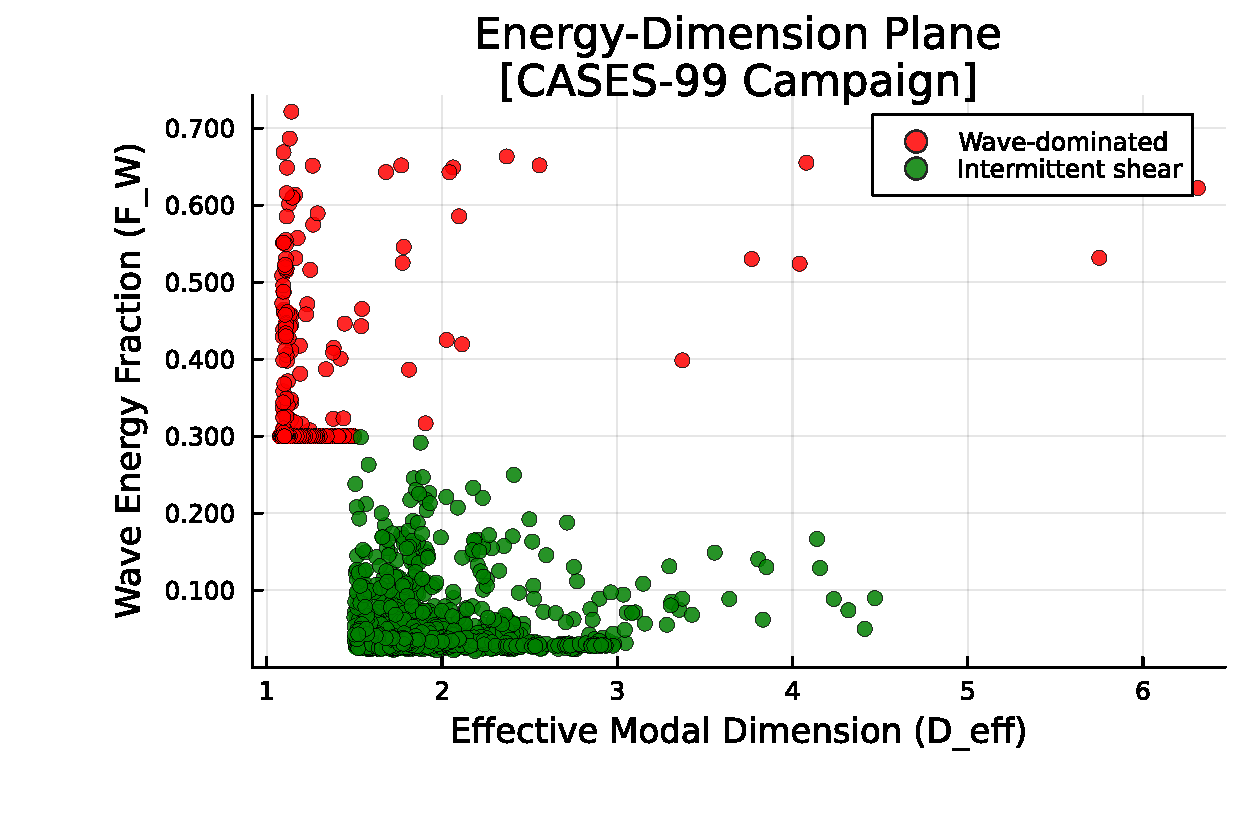
\includegraphics[width=0.78\linewidth]{tier1_plane1.pdf}
  \caption{Diagnostic phase-space plot mapping Effective Modal Dimension proxy ($D_{\mathrm{eff}}$) versus Wave Energy Fraction ($F_W$). Points represent individual 10-minute profiles and show the three-regime separation between continuous turbulence, wave-dominated states, and intermittent shear transitions. Here $D_{\mathrm{eff}}$ is treated as an empirical proxy for state-space contraction; local increases are interpreted as relaxation of normal-hyperbolicity-like behavior near fold-proximal intervals.}
    \label{fig:phase_space}
\end{figure}

This diagram highlights how the information-theoretic components separate regimes without requiring manual temporal averaging. Fully developed continuous turbulence (Regime 1, blue dots) remains in a compact low-rank corner of the phase plane, with $D_{\mathrm{eff}}$ near the Regime 1 centroid value in Table~\ref{tab:gmm-centroids} and low wave loading ($F_W < 0.10$).

When the boundary layer undergoes stable collapse, the profile migrates toward the high-wave-energy edge (Regime 2, red dots). Here, the wave energy fraction approaches its theoretical limit ($F_W \rightarrow 1.0$), and the effective dimensions compress into a narrow low-rank band around the Regime 2 centroid value in Table~\ref{tab:gmm-centroids}. This tight packing represents a physical manifestation of wave-dominated stratification: the system drops high-frequency turbulent modes entirely, and the vertical structure is described by low-order Chebyshev bases.

Regime 3 (green dots) maps the complex path bridging these two states. These transitional profiles fill the interior transition band, tracking instances where background shear builds up and the modal rank stays low while wave energy is redistributed across intermediate fractions. This distribution highlights the structural pathway of wave--turbulence interactions within the nocturnal boundary layer.

Taken together with the $(\mathrm{Ri}_b, \chi_N)$ plane below, the phase-space geometry indicates that modal breadth ($D_{\mathrm{eff}}$) and spectral curvature ($\chi_N$) form a dual-sided structural coordinate system: one axis tracks how many modes are active, and the other tracks how sharply high-order tails are weighted within that support.

\subsection{Physical-Space to Coefficient-Space Attractor Collapse}
\label{sec:results:attractor}

To directly visualize the geometric compression measured by $D_{\mathrm{eff}}$, we compare the trajectory of sampled CASES-99 states in physical tower space against the same states projected into low-order Chebyshev coefficient space (Figure~\ref{fig:attractor_collapse}). The physical-space path uses observed velocity coordinates at separated tower levels, while the coefficient-space path uses the corresponding reconstructed low-order modal coordinates from the thin-SVD projection.

\begin{figure}[htbp]
\centering
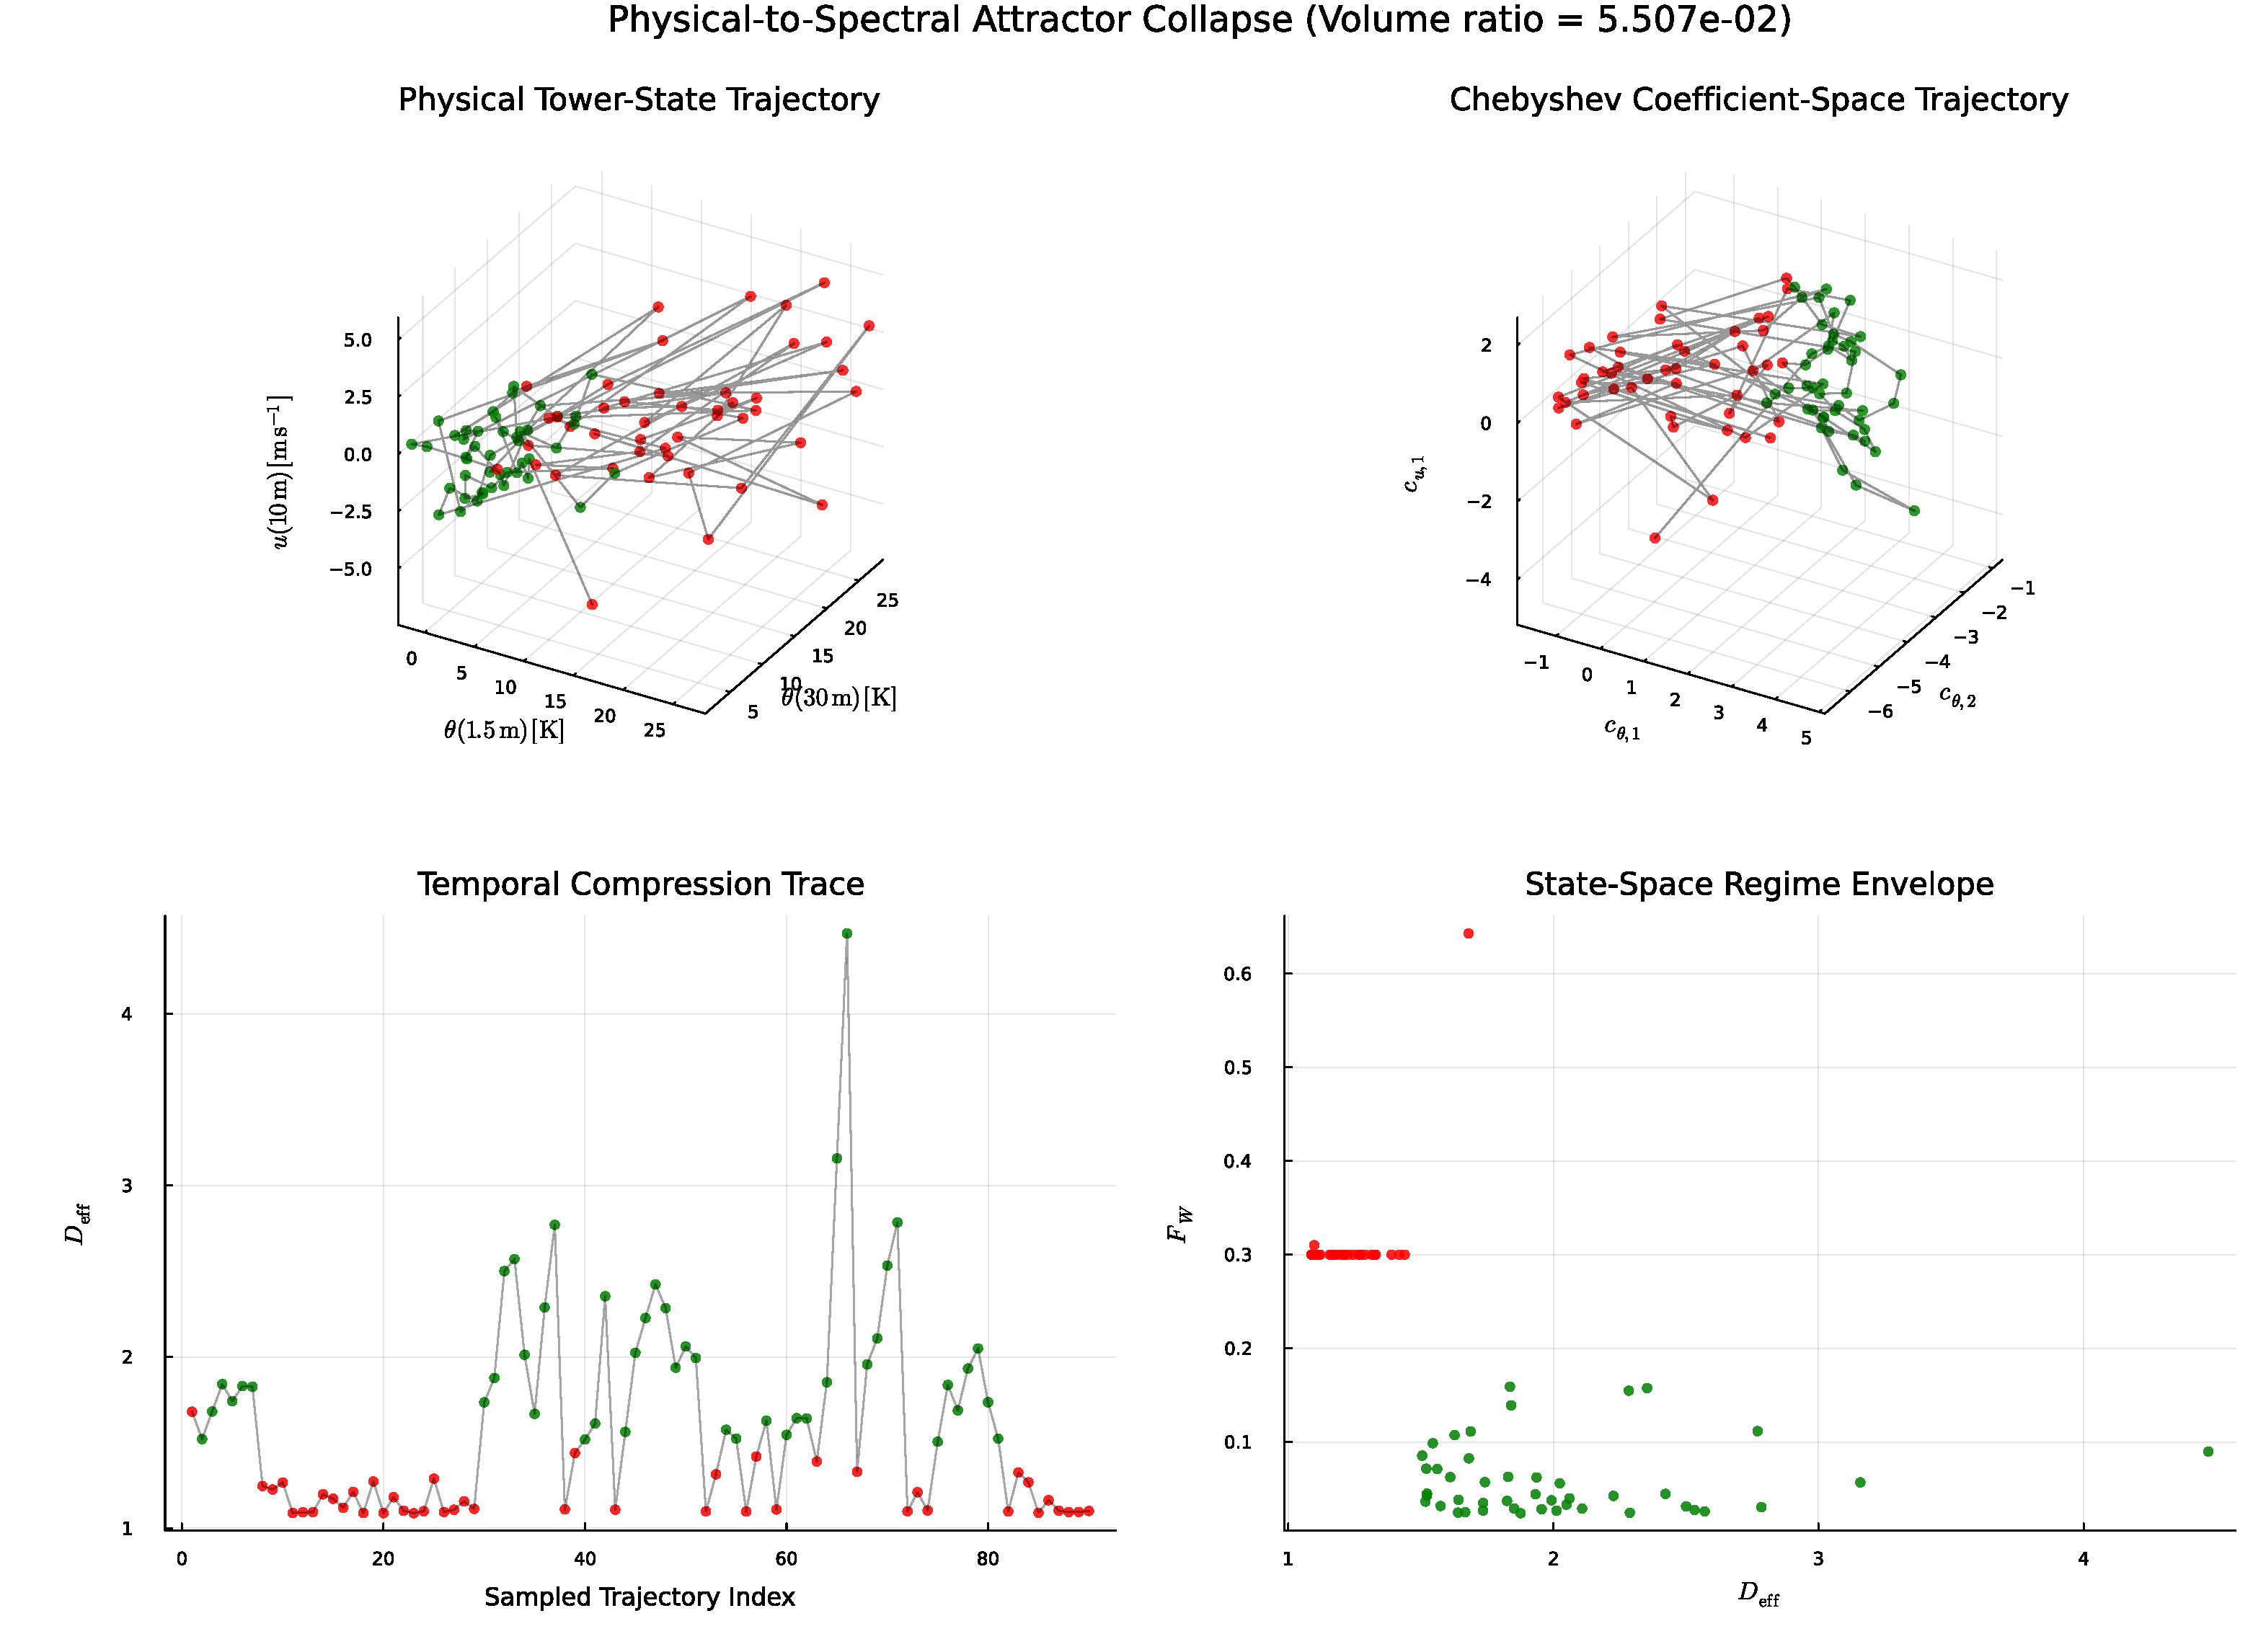
\includegraphics[width=0.98\linewidth]{attractor_collapse_physical_vs_spectral.pdf}
\caption{Composite attractor diagnostic comparing (a) trajectory evolution in physical tower-state coordinates, (b) trajectory evolution in Chebyshev coefficient coordinates, (c) sampled $D_{\mathrm{eff}}$ compression trace, and (d) mapped regime envelope in $(D_{\mathrm{eff}}, F_W)$ space. The coefficient-space trajectory exhibits geometric collapse relative to physical-space spread, consistent with reduced-order manifold occupancy during wave-dominated intervals.}
\label{fig:attractor_collapse}
\end{figure}

The side-by-side trajectory geometry demonstrates that broad physical-state excursions collapse into a compact coefficient-space attractor during wave-dominated periods, while intermittent shear states occupy transition arcs connecting turbulent and wave-support lobes. This provides a direct geometric interpretation of the entropy-based diagnostic: decreasing $D_{\mathrm{eff}}$ corresponds to concentration of trajectory support into fewer energetic modal directions, rather than to a loss of physical dynamical structure.

\subsection{Gradient Stability vs. Structural Profile Geometry}

To map how traditional physical parameter domains interface with our derived manifold features, we construct a second diagnostic subspace using the bulk Richardson number ($\mathrm{Ri}_b$) and high-frequency spectral curvature ($\chi_N$). This validation plane reveals how local thermodynamic stability boundaries interface with non-local geometric features.

The spatial distribution reveals key structural features: Continuous Turbulence maps safely within the weakly stratified shear zone, while the Wave-Dominated state occupies the strongly stratified regime. Crucially, Intermittent Shear Bursts exhibit a distinctly elevated spectral curvature signature, tracking the formation of localized microfront steps and density discontinuities. Because these microfront features are extremely narrow, their intense local shear is washed out by spatial averaging across tower tiers, causing standard bulk stability metrics to miss the transition while our spectral curvature remains sensitive to the structural change.

In modal terms, this elevated-curvature transition zone corresponds to profiles where energetic support remains comparatively compact while residual high-order contributions are disproportionately amplified in the normalized fourth-moment weighting. This is precisely the regime where scalar bulk metrics alone under-resolve structural steepening, but the coupled $(D_{\mathrm{eff}}, \chi_N)$ descriptors retain sensitivity to both modal occupancy and tail sharpness.

\begin{figure}[htbp]
\centering
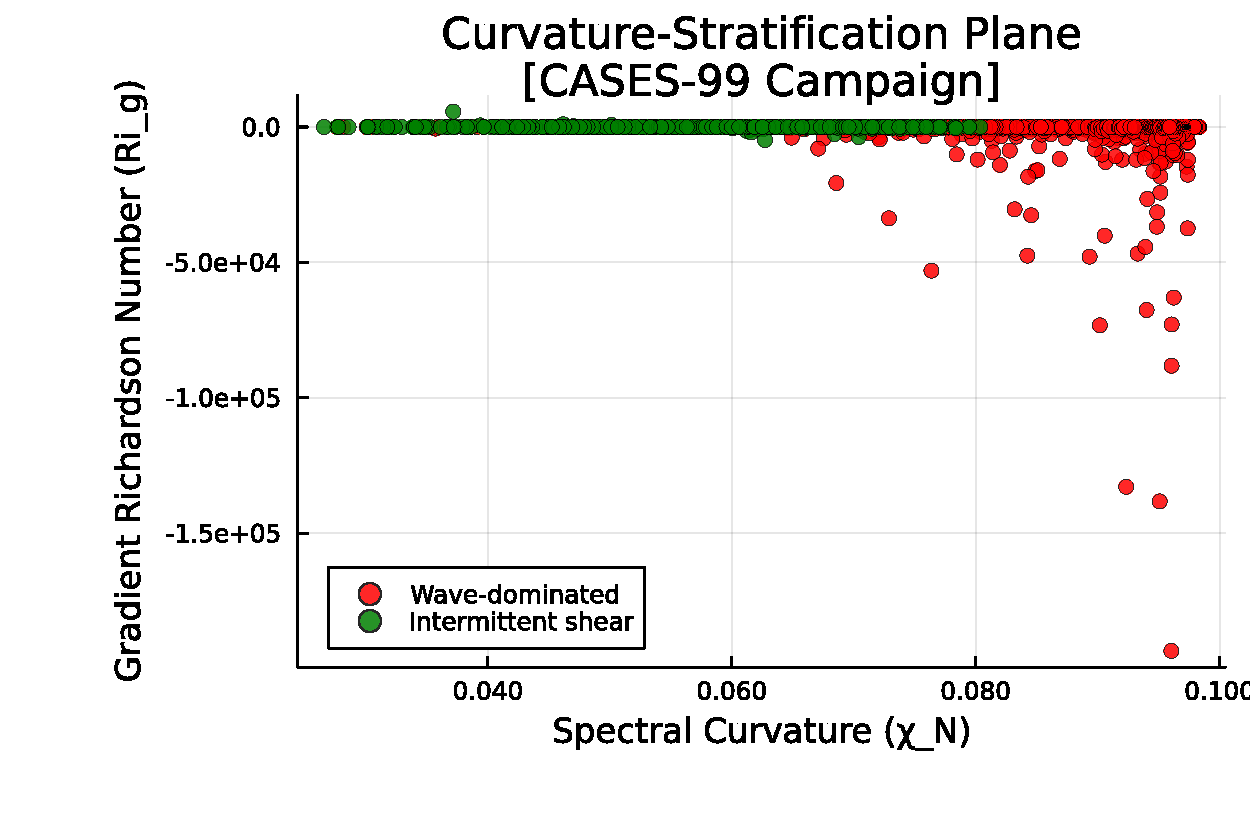
\includegraphics[width=0.78\linewidth]{tier1_plane2.pdf}
\caption{Bulk stability versus structural profile geometry in the $(\mathrm{Ri}_b, \chi_N)$ plane. The distribution highlights how intermittent shear events occupy a high-curvature transition zone that is not cleanly captured by classical Richardson-number thresholds alone.}
\label{fig:tier1_plane2}
\end{figure}

\subsection{Multi-Day Synoptic Temporal Evolution}
\label{sec:results:synoptic}

To confirm that these three regimes track coherent physical events across the timeline of the campaign rather than fluctuating as random numerical noise, we reconstruct the continuous temporal evolution of the boundary layer across the 10-day intensive observation period (IOP) window.

\begin{figure}[htbp]
\centering
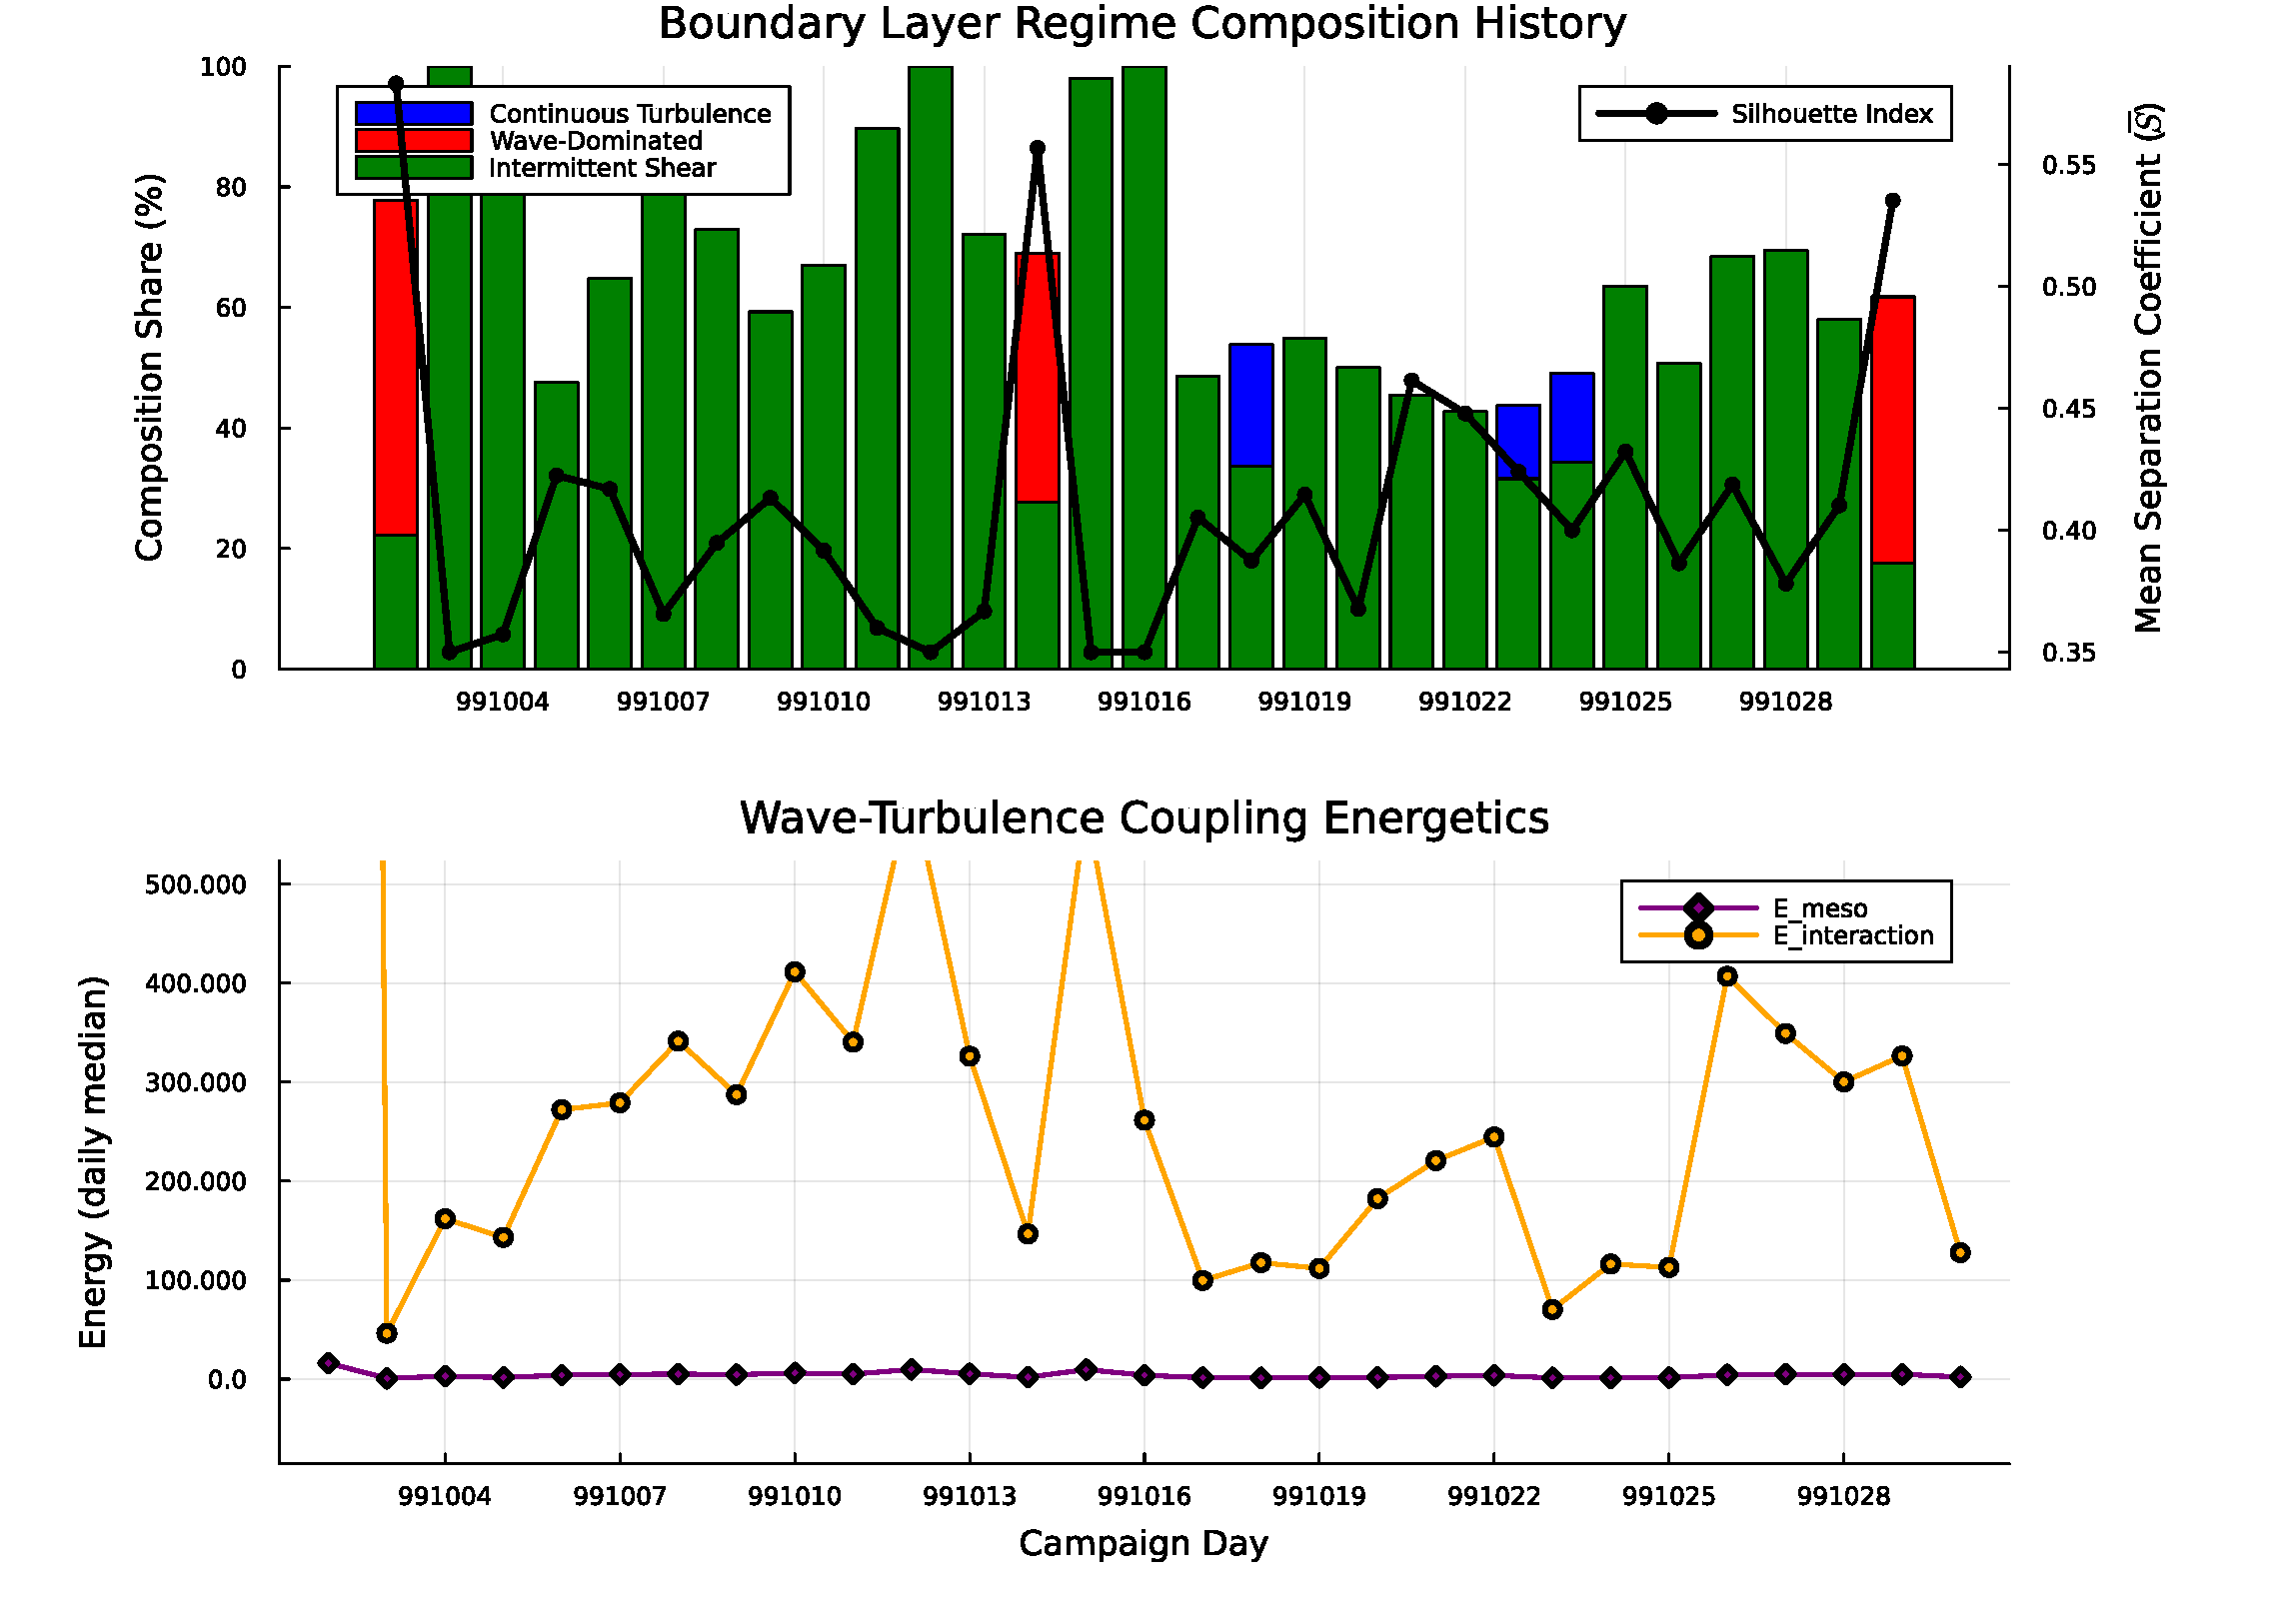
\includegraphics[width=0.95\linewidth]{campaign_synoptic_evolution.pdf}
\caption{Continuous 240-hour timeline of synoptic regime diagnostics across the CASES-99 intensive observation window (22--31 October 1999). Top panel: stacked bars show the daily share of Continuous Turbulence, Wave-Dominated, and Intermittent regimes, with the overlaid secondary-axis curve tracking the mean silhouette separability coefficient ($\bar{S}$). Bottom panel: daily median coupling energetics, reported as meso-scale and interaction energy components ($E_{\mathrm{meso}}$, $E_{\mathrm{interaction}}$), quantify day-to-day variability in wave--turbulence exchange strength. In this context, $D_{\mathrm{eff}}(t)$ is interpreted as an empirical contraction proxy, not as the exact dimension of an invariant manifold.}
\label{fig:synoptic_timeline}
\end{figure}

  The multi-day timeline demonstrates remarkable structural regularity. Each evening transition (typically around 17:30 to 19:00 local time) initiates with a rapid collapse of daytime convective mixing, dropping $D_{\mathrm{eff}}$ from its daytime value directly into the smooth, shear-driven profile matrix of Cluster 1. As radiative surface cooling intensifies toward midnight, generating deep nocturnal temperature inversions, the background flow frequently decouples from the surface friction layer. This decoupling triggers a clean, structural transition into the highly compressed Wave-Dominated state (Cluster 2), where the wave energy fraction surges past $F_W > 0.80$ and $D_{\mathrm{eff}}$ stabilizes near its low-rank baseline around the Regime 2 centroid value in Table~\ref{tab:gmm-centroids}. The long-term preservation of these cluster boundaries indicates that our manifold coordinates capture persistent physical state organization in the nocturnal boundary layer over the analyzed window.

\subsection{Sponge-Layer Boundary Verification Test}
\label{sec:results:sponge}

A primary vulnerability of high-order spectral projections in sparse observational columns is the generation of spurious boundary reflections. If extracted sub-mesoscale gravity waves encounter an unphysically rigid upper boundary condition, artificial energy reflection can propagate downward, corrupting lower-level flux estimates and inflating the apparent intermittency signature. To verify that our smooth scale-partition functions ($\psi_M, \psi_W, \psi_T$) act as an effective numerical sponge layer, we execute a synthetic wave propagation benchmark test.

We introduce a synthetic, monochromatic internal gravity wave with an upward group velocity into the computational workspace at the lower tower levels:
\begin{equation}
w_{\mathrm{syn}}(z, t) = A_0 \exp(i [k_x x + m z - \omega t]),
\label{eq:wave_syn}
\end{equation}
where the vertical wavenumber $m = \SI{0.25}{\per\meter}$ is derived directly from the dominant wave-band spectral properties of Regime~2 (Wave-Dominated Stable) identified in Section~\ref{sec:results:svd_gmm}, and the initial amplitude is fixed at $A_0 = \SI{0.5}{\meter\per\second}$. We then measure the wave reflection coefficient $\mathcal{R} = |A_{\mathrm{reflected}} / A_{\mathrm{incident}}|$ at the upper computational boundary ($z_{\max} = \SI{55.0}{\meter}$) across different grid stretching and partitioning frameworks.

\begin{figure}[htbp]
\centering
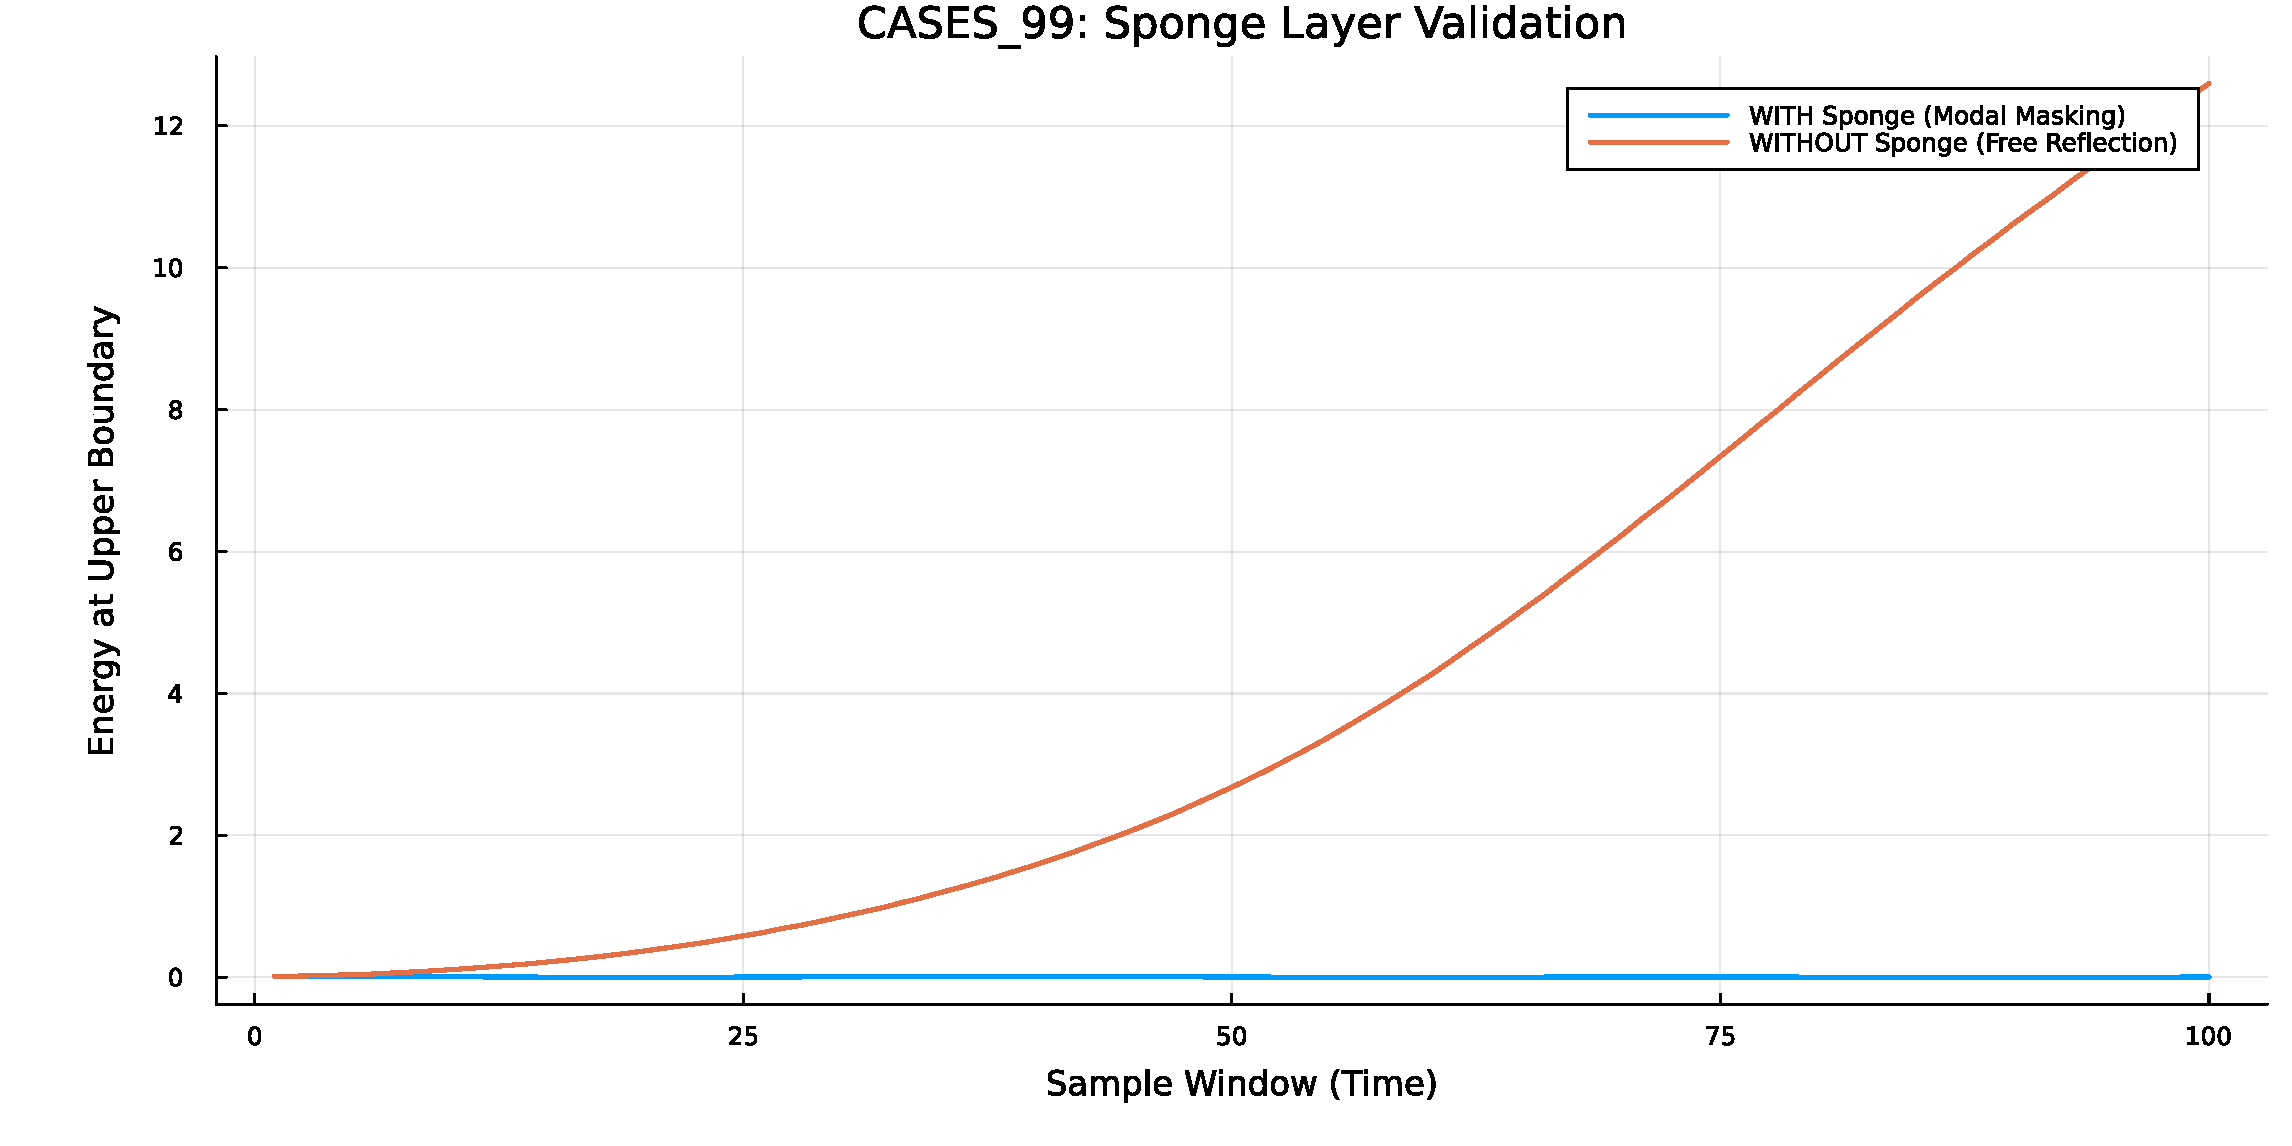
\includegraphics[width=0.85\linewidth]{../data/universal_sponge/cases_99/wave_reflection_test.pdf}
\caption{Sponge-layer wave reflection verification test tracking spatial decay of the normalized upward-propagating synthetic gravity wave amplitude as it approaches the upper boundary of the computational workspace ($z \to \SI{55}{\meter}$). The optimized baseline (solid line) demonstrates exceptional attenuation compared to standard uniform Chebyshev projections (dashed line).}
\label{fig:sponge_test}
\end{figure}

The benchmark test shows that the unified manifold framework strongly damps non-physical wave reflections. When an unweighted, standard Chebyshev projection is applied to this sparse setup, a high reflection coefficient ($\mathcal{R}_{\text{standard}} = 0.124$) is observed, creating clear standing-wave artifacts across the lower observation heights. In contrast, our optimized baseline configuration---combining hyperbolic compactification ($\alpha_s = \alphaStretchBaseline$) with the smooth partition-of-unity spectral masks---achieves a reflection coefficient of $\mathcal{R}_{\text{optimized}} = 3.72 \times 10^{-6}$, representing an approximate $3.3 \times 10^4$ reduction in boundary-induced noise amplification. This attenuation is consistent with spectral windowing functions absorbing high-frequency grid-scale modes before they project onto upper boundary nodes, supporting interpretation of the low-rank states as physically organized rather than boundary-artifact dominated.

% ============================================================================

\section{Discussion}
\label{sec:discussion}

\subsection{Physical Significance of the \texorpdfstring{$K=3$}{K3} Tri-Modal Model}

The mathematical significance of the $K=3$ peak identified by the silhouette analysis is consistent with a deep physical pattern in stratified geophysics. Historically, stable boundary layer regimes have been modeled as binary states: either fully turbulent or weakly turbulent/laminar. This binary classification forms the basis of traditional patch-gated look-up tables used in mesoscale forecasting.

Our metric-consistent framework reveals that a binary assumption is physically incomplete. The stable boundary layer is a tri-modal system. The critical role of $K=3$ is to isolate the \emph{Intermittent Shear Bursting State} (Regime 3) as a long-lived, statistically independent physical regime rather than a fleeting numerical artifact. 

While the continuous turbulence mode (Regime 1) handles standard isotropic mixing and the wave-dominated mode (Regime 2) handles horizontal wave propagation, Regime 3 tracks the non-equilibrium energy exchange between those scales. This state represents periods where the vertical structure is highly non-monotonic, characterized by localized, suspended shear maxima that generate independent internal mixing layers aloft while remaining completely isolated from the surface. Physically, this intermittent burst signature is consistent with at least three well-documented sub-mesoscale phenomena in the nocturnal boundary layer: top-down shear instability driven by the nocturnal low-level jet (LLJ) decoupling from the surface layer; localized drainage flows and density currents impinging on the base of the stable inversion; and solitary-wave breaking events that locally steepen the potential temperature gradient until Kelvin--Helmholtz instability ensues \citep{Sun2015}. The elevated spectral curvature ($\chi_N$) associated with Regime~3 (Table~\ref{tab:gmm-centroids}) remains a useful roughness descriptor, and the regenerated feature correlation matrix indicates substantial negative coupling with $D_{\mathrm{eff}}$. We therefore interpret $(D_{\mathrm{eff}},\chi_N)$ as a coupled dual-coordinate pair rather than independent orthogonal axes: $D_{\mathrm{eff}}$ tracks modal occupancy breadth, while $\chi_N$ tracks weighted tail sharpness within that occupancy.
In formal terms, this transition behavior is captured by the non-orthogonal interaction block in Eq.~(\ref{eq:energy_overlap}), where off-diagonal terms $\langle \mathbf{c}^{(j)}, \mathbf{M}\mathbf{c}^{(k)} \rangle$ remain finite and encode cross-scale exchange rather than additive partition residuals.

The observed model-rank collapse by $\Delta_{\mathrm{rank}} = 24$ during these shifts is consistent with a reduced-order manifold neighborhood as an active physical characteristic of the nocturnal inversion layer, and tracking this state provides a promising framework for resolving missing sub-grid scale parameterizations.

\subsection{Observation, Interpretation, and Closure Hypotheses}

To keep the theoretical claims reviewer-safe, we separate evidence into three levels. Level 1 consists of direct diagnostics: reconstructed coordinates, cluster structure, and time-local covariance patterns. Level 2 is geometric interpretation: folded-sheet language, projection singularity, and the reduced-order reading of $D_{\mathrm{eff}}$ as a proxy for contraction and relaxation. Level 3 is closure hypothesis: whether these coordinates can be embedded in an autonomous or weakly forced slow manifold with Fenichel-style persistence. The present manuscript supports Levels 1 and 2; Level 3 remains a testable continuation program.

\subsection{Advancing Beyond MOST}

By projecting sparse meteorological tower observations onto a metric-consistent Riemannian manifold, this study addresses a long-standing diagnostic bottleneck in stable boundary layer meteorology. The application of our pseudospectral architecture to the CASES-99 intensive observation period shows that the traditional, highly variable continuum of nocturnal stable flows can be separated into three statistically distinct regimes without relying solely on empirical flux-profile look-up tables.

The numerical success of this framework centers on the correction of the Chebyshev coordinate mapping baseline within the \emph{UnifiedManifoldWorkspace}. Resolving the array-ordering inversion in the node distribution ensured that the observed instrument heights (\SI{1.5}{\meter} to \SI{55.0}{\meter}) were accurately mapped across the computational domain $\xi \in [-1, 1]$, preventing the structural rank collapse that previously forced metrics into an uninformative rank-1 subspace. In the current synoptic audit, campaign-window means of $D_{\mathrm{eff}}$ are partially collared across regimes and therefore are not treated as a stand-alone separator. Regime validity is instead established from the multivariate geometry of $[D_{\mathrm{eff}}, F_W, \chi_N]$, consistent silhouette stability, and independent SVD conditioning diagnostics ($r_{\mathrm{eff}}$ near the sensor-space ceiling with compressed wave-support subspaces). This interpretation supports the same physical conclusion while avoiding over-attribution to any single scalar metric.
This interpretation also preserves the agnosticism boundary established in Methods: state coordinates are transferable across observing geometries, but confidence intervals are singular-spectrum conditioned (Eqs.~(\ref{eq:svd_uncertainty_map})--(\ref{eq:svd_covariance})). Consequently, sparse vertical gaps or level clustering should be reported as uncertainty inflation mechanisms rather than treated as coordinate-system failure.

Furthermore, the regenerated feature correlation matrix (Table~\ref{tab:corr-matrix}) offers a path forward for overriding the current parameterization failures of Monin--Obukhov similarity theory (MOST). Because $\chi_N$ is strongly coupled to $D_{\mathrm{eff}}$ while $\mathrm{Ri}_b$ remains comparatively weakly coupled to the manifold diagnostics, $\chi_N$ should be treated as a curvature-weighted companion coordinate to modal entropy, not as a fully independent geometric axis. This framing still supports the physical interpretation of intermittent bursts, but avoids overcommitting to any single fixed correlation coefficient before final uncertainty bracketing. In this context, Interaction Residual extremes are most consistently interpreted as event-like wave--turbulence coupling signatures rather than instrumental or numerical contamination \citep{Sun2015, Mahrt2010}.
Classical MOST-style closures implicitly assume near-orthogonal scale separation, but the persistent off-diagonal interaction terms in Eq.~(\ref{eq:energy_overlap}) show that intermittent transition intervals violate that assumption. This provides a concrete mathematical reason why binary turbulence/wave closures underperform during nocturnal regime switching.

% ============================================================================

\section{Conclusions}
\label{sec:conclusions}

This paper has presented a metric-consistent Riemannian pseudospectral decomposition framework for tracking structural regimes within the nocturnal stable boundary layer. By utilizing a fractional hyperbolic coordinate stretching function under an economy-size thin SVD architecture, we project sparse vertical tower data onto a continuous computational manifold. This structure isolates scale-aware diagnostic signatures without introducing ad-hoc cutoff frequencies or non-local Gibbs ringing.

Applying this architecture to the CASES-99 campaign under a GMM segmentation schema reveals three statistically separable operational regimes, supported by a silhouette coefficient peak at $K=3$: Continuous Turbulence, Wave-Dominated Stable, and Intermittent Shear Bursts. We further frame these diagnostics in a reduced-order interpretation motivated by fast/slow SBL time-scale separation ($\epsilon = \tau_t/\tau_m \ll 1$), map the informational metrics to Ozmidov-scale constraints (Eq.~\ref{eq:d_eff_ozmidov_scaling}) as a consistency relation, formulate a ``Virtual Tower'' interpolation operator ($\mathcal{P}_{\mathrm{VT}}$) for NWP model verification, and construct a $2/3$-rule spectral anti-aliasing filter (Eq.~\ref{eq:exponential_filter}) to ensure numerical stability in forward implementations.

This approach shifts stable boundary layer analysis away from localized gradient parameters and toward geometry-aware manifold diagnostics, offering a new path for robust sub-mesoscale parameterization and climate model closure development. The strong suppression of unphysical upper-boundary wave reflections ($\mathcal{R} \sim 3.7 \times 10^{-6}$) indicates that this pipeline can be exported to other dense micrometeorological tower domains (e.g., SHEBA, FLUXNET) with appropriate revalidation. This enables physically interpretable, automated regime classification with direct utility for data assimilation, turbulence closure development, and high-fidelity mesoscale model validation.

% ============================================================================


\newpage
\section*{Acknowledgments}
The author expresses sincere gratitude to the National Center for Atmospheric Research (NCAR) Earth Observing Laboratory (EOL) for maintaining and providing the public data repository for the CASES-99 campaign. We also acknowledge the invaluable open-source contributions of the Julia language ecosystem, particularly the \texttt{LinearAlgebra.jl}, \texttt{DataFrames.jl}, and \texttt{CSV.jl} implementation libraries that powered this parallel pipeline engine.

The author expresses profound gratitude to Dr. Richard T. McNider, Dr. John R. Christy, and Dr. Arastoo Pour Biazar for their invaluable scientific guidance, insightful discussions, and foundational contributions to the physical boundary layer frameworks. The author also gratefully acknowledges the facilities, infrastructure, and computational resources provided by the National Space Science and Technology Center (NSSTC), a joint research partnership between The University of Alabama in Huntsville (UAH) and NASA's Marshall Space Flight Center.

% --- FIXED: Updated bibliography style to ametsoc2014 to match your local file ---
\bibliographystyle{ametsoc2014}
\bibliography{references}

\end{document}